\chapter{Galaxyfly:一种新型大规模灵活阶数的高性能互连网络低直径拓扑结构设计}

\section{引言}
当前大规模高性能计算机系统已达几万个计算节点的规模,
如“$神威\cdot 太湖之光$”系统和天河二号系统。
高性能计算机系统规模仍然在增长,预计2023年推出的E级系统,
规模将达到几十万规模的计算节点。
互连网络对高性能计算机系统的扩展起到重要作用并影响整个系统的设计。
其中,互连网络最重要的设计是拓扑结构。
拓扑结构限制了网络的理论上限(如:端到端的延迟和二分带宽)和决定了网络的成本开销。

为下一代大规模高性能计算机设计一个有效的拓扑结构需要考虑几个指标。
第一,高带宽和低延迟一直是优化网络拓扑结构的重要目标。
第二,一个有效的拓扑结构不仅成本开销经济而且能耗开销也要考虑在内。
能耗开销和整个系统的成本开销都有严格的限制,
如:E级系统的能耗需要限制在20-30MW以内\upcite{nextplatform}。
其中,网络构建成本开销和能耗开销分别能够达到整个系统开销的
$33\%$\upcite{Flattenedbutterfly} 和$50\%$\upcite{Energy}。
最后一点,灵活性也是一个有效拓扑结构的重要指标。
一个以应用为主的高性能计算系统设计\upcite{Reconfigurable},
互连网络通过静态布局或者动态配置可以适应不同规模的应用和通信需求。

当前大多数的研究都关注在设计低直径的拓扑结构,
同时优化成本和其他指标。一些优秀的低直径拓扑结构被提出,
如Flattened Butterfly\upcite{Flattenedbutterfly}、Dragonfly\upcite{dragonfly}、
HyperX\upcite{hyperx}、Skywalk\upcite{skywalk} 和Slim Fly\upcite{slimfly}。
这些拓扑结构虽然能够提供较低的网络直径,
但是扩展至E级系统甚至规模更大的网络仍然很困难。
主要限制他们扩展性的是因为路由器的端口数。
增加路由器端口数并满足当前高阶拓扑结构达到E级计算规模对当前乃至未来几年的
商用路由器设计都是困难的。
48端口的路由器\upcite{omni}是当前最新的商用模块,
并计划应用在2018 年Argonne实验室、
Cray公司以及Intel公司联合推出的180Pflops的高性能计算机系统。
芯片的物理资源和能耗开销是两个限制端口数增长的重要指标\upcite{roleoptics}。
在电信号路由器芯片上,增加端口数的同时维持或增加每个端口的带宽就会
授限制于交换crossbar的连线复杂度和芯片边缘的带宽密度\upcite{roleoptics}
以及高速SerDes 的I/O。
很多研究者根据这些挑战提出了很多高阶路由器模型,
如64端口的基于瓦片的YARC 交换机\upcite{blackwindow}、
64端口的2D Swizzle-switch\upcite{swizzle}、
64 端口的3D Hi-Rise交换机\upcite{hirise}和136端口的SCOC交换机\upcite{scoc}。
但是,这些产品应用到实际系统中还需很长的一段时间。
比如说,SCOC的每个端口的速率25Gbps\upcite{scoc},
略低于现在商用的路由器,
如48端口的Intel Omni-Path交换芯片和36端口的Mellanox公司推出的EDR InfiniBand交换芯片。
而且,bytes-to-flops的比例关系到每个节点的网络通信总量和浮点运算能力,
这是均衡网络的重要标志。一个计算节点的链路带宽随着计算能力而有比例的增加。
为了满足前沿网络的需求,网络传输速率已经开始采用200Gbps的技术\upcite{road200G}。
当前最先进的200G交换芯片是由Mellanox公司推出的HDR InfiniBand交换芯片,
但也只有40 个端口\upcite{quantum}。
增加高阶路由芯片端口数的同时增加端口带宽是非常困难的。
硅光子技术被期望来解决这些困难。
Altera和Avago已经设计出一种基于嵌入并行光模块的光信号FPGA\upcite{avagotech}。
但是,在一块芯片上集成容纳足够的光模块仍然是很困难的工作。
端口数增加的同时也会增加芯片的能耗开销。
例如,在天河二号计算系统中一条SerDes 链路传输一个比特需要消耗20pJ,
而且SerDes的能耗开销占一个芯片的总开销的$79\%$\upcite{Liao2015}。
而且,物理封装设计面积和热量的限制将要严重影响高速SerDes
的数量以及路由器端口数的密度\upcite{road200G}。
因此,E级互连网络设计将要面对路由器端口数影响扩展性的问题。

大多数已有的工作都是关注高阶拓扑结构,
如Fat tree、Flattened Butterfly\upcite{Flattenedbutterfly}、Dragonfly\upcite{dragonfly}、
HyperX\upcite{hyperx}、Skywalk\upcite{skywalk} 和Slim Fly\upcite{slimfly}等。
高阶拓扑结构相比低阶拓扑结构(如:Torus和Mesh结构)可以获得更低的网络延迟。
Fat tree是一个经典的高阶间接网络,
同时也可以通过增加层数使用较低阶的路由器搭建大规模网络,
但是这样会消耗大量链路和路由器。Dragonfly结构不仅网络直径低,
而且结合了光链路和电链路的优势减少网络开销。
但是,使用当前最新推出的商用高阶路由芯片
(如:48端口的Intel Omni-Path 交换芯片\upcite{omni})
来构建Dragonfly 结构仍然不能达到100K 规模。
实际上,Dragonfly结构的扩展性问题限制了他在实际系统中的部署。
比如,Cray公司的Cascade系统\upcite{cascade}采用的是变形的Dragonfly结构,
为了增强结构的可扩展性,
组内结构不是标准定义的全互连结构而是2维的Flattened Butterlfy 结构。
Dragonfly+\upcite{Dragonfly+}是被提出来扩展传统Dragonfly结构
通过树型结构代替超级节点内的全互连结构并且支持相近的性能。
在使用相同端口数的路由器,Dragonfly+的规模可以达到Dragonfly规模的常数倍。
在给定的网络规模,Dragonfly+使用的路由器端口数可以减半但是路由器数量翻倍。
HyperX 可以灵活调整参数配置,是一个灵活的拓扑结构。
其每一维上是一个全互连的结构,非常适合使用光链路互连。
Flattened Butterfly 和Hypercube都是HyperX 结构的特例。
但是,HyperX的最大问题就是每一维上全互连的结构会大大影响网络的扩展和增加网络的开销。
随机拓扑结构\upcite{acaserandom}\upcite{layoutrandom}\upcite{Jellyfish}
提供了不一样的设计空间和满足递增式的扩展,
无论多大规模路由器端口数有多少都可以构造出来。
然而,随机拓扑结构的路由算法和链路拥塞是随机拓扑结构的最大问题。
Slim Fly采用了详细的图论知识构造一个近似Moore bound 规模的网络。
Slim Fly的目标就是完成在给定节点度数和网络直径为2的条件下构造尽可能大规模的结构。
然而,Slim Fly的扩展性受限制于他的低延迟和路由器端口数。
一旦路由器端口数不再增加,
那么我们不得不重新权衡节点度和网络直径即网络性能和网络可扩展性
对高阶拓扑结构设计的影响。

除了这些高性能计算系统的拓扑结构,数据中心系统的拓扑结构也值得高性能计算系统借鉴。
Xpander\upcite{xpander}是最近提出的类似随机网络性能的规则结构。
而且,Xpander可以递增的扩展并可以很好的管理缆线。
但是,Xpander结构内的连线是不确定的,
仍然面临路由表规模大的问题。
Dcell\upcite{dcell}和Bcube\upcite{bcube}都是层次化网络。
Dcell是一个迭代结构而且随着节点度的增加规模呈指数倍扩展。
Bcube是一个以终端为中心的网络结构即终端的网卡接口数增加网络规模增加。
因此,Dcell 和Bcube不能很好的支持灵活扩展。
一些可配置的网络结构被提出通过增加自由光链路\upcite{fso}
或者无线链路\upcite{FireFly}来满足不同应用和扩展性的需求。
但是,这种拓扑构建的设备成本和环境要求高于别的拓扑结构。

本章节目标就是使用有限的路由器端口数构造E级计算系统。
我们设计了灵活阶数的低直径网络并权衡了节点度和网络直径的关系。
我们最主要的目标就是使用当前商用路由器构造互连网络。
进一步的目标就是增加结构的灵活性,
以至于该拓扑结构可以灵活调整网络规模和二分带宽,
使得结构可以部署从P级系统到E级系统规模,甚至更大规模的网络。
我们设计了一类新的低直径拓扑结构,Galaxyfly。
Galaxyfly利用代数图论有限域的方法降低了对高阶路由器端口数的要求并可以通过不同的配置灵活扩展。
Galaxyfly权衡好网络规模和二分带宽的关系后仍然能够维持一个较小的网络直径。
而且,Galaxyfly采用代数图论的性质可以促使我们设计延迟敏感的路由算法。
另外,Galaxyfly是一个灵活的层次化拓扑结构,
由Galaxy图和全互连图两个模块组成。
这两个模块很好的利用了芯片间光互连和背板之间的互连技术,
并易于物理布局。
Galaxlyfly灵活的层次结构也使得其能够支持不同的通信模式,
比如:局部的全互连适用局部的密集通信以及全局的冗余链路可以自适应的满足集中的全局通信。
其中,Dragonfly和全互连结构都是Galaxyfly的特例。

本章的主要贡献如下:

$\bullet$我们定义了一种新的结构,Galaxy图。
Galaxy图的直径最多为2。
我们设计和分析了基于Galaxy图和全互连图组合而成的Galaxyfly结构。
另外,我们比较了Galaxyfly结构与其他拓扑结构在灵活性、可构造配置以及最短路径和
容错性等指标上的性能。

$\bullet$利用Galaxy图,
我们设计了最短路径路由和其他非最短自适应路由算法并比较了Galaxyfly 的不同配置下与
其他拓扑结构在物理布局下的性能。

$\bullet$相比其他经典拓扑结构,
Galaxyfly因为灵活的物理布局特性减少了成本开销和能耗开销。

\section{Galaxyfly拓扑结构}

在这一章节,我们介绍一个灵活可配置的图,Galaxy图。他的构造源于代数图以及他的网络直径最多为2。
基于Galaxy图,我们设计了一类低直径拓扑结构,Galaxyfly。他不仅能够降低扩展性对路由器端口数
的需求而且很好的权衡网络规模和二分带宽的关系。

\subsection{Galaxy图}

我们的目标是使用固定的路由端口数搭建更大的网络规模并降低对路由器数量的需求和网络直径。这是一个类似经典Moore 图
的问题。与Slim Fly\upcite{slimfly}相似,我们采用了McKay等人在文献\upcite{NLG} 中介绍的图论技术构造了基本
模块直径为2的Galaxy图。那些近似Moore bound直径为2的图技术有助于设计Galaxy 图并有效证明Galaxy图的网络直径
最多为2\upcite{NLG}。在本小节剩余的部分我们将介绍Galaxy图的构造和证明Galaxy 图的直径最多为2。

Galaxy图是一个规模为$n\times q$的图$G(V,E)$,而且可以等价的划分为$n$个集群,$V= V_{0}\cup V_{1}\cup \cdots \cup V_{n-1}$。
每个集群$q$个节点。$q$是一个素数幂并满足$q=4\ell+\delta$, $\delta\in\{-1,0,1\}$。

在介绍Galaxy图构造方法之前,先介绍一些代数图和有限域的相关知识。相关概念里所有的
算术操作都需要进行模$q$的运算。

$q$产生一个有限域$\mathds{F}_q=\{x_{0},x_{1},...,x_{q-1}\}$。 其中,$\mathds{F}_q^+$是他的加法群。
我们可以找到有限域$\mathds{F}_q$
的生成元$\xi$, 他属于$\mathds{F}_q$并生成$\mathds{F}_q$
以$\{\xi^t mod\ q | t \in \mathds{N}\}$的形式。两个生成集$X$和$X'$,通过生成元$\xi$构造,
如等式\eqref{equ:generator-sets0}和\eqref{equ:generator-sets1}所示:

\begin{equation}\label{equ:generator-sets0}
  X=
  \begin{cases}
    \{1,\xi^2,\ldots,\xi^{q-3}\}& q=4 \ell+1 \\
    \{1,\xi^2,\xi^4,\ldots, \xi^{2\ell-2},\\\xi^{2\ell-1},\xi^{2\ell+1},\ldots, \xi^{4\ell-3}\} & q=4 \ell-1 \\
    \{1,\xi^2,\ldots,\xi^{4l-2}\} & q=4 \ell
  \end{cases}
\end{equation}

\begin{equation}\label{equ:generator-sets1}
  X'=
  \begin{cases}
    \{\xi,\xi^3,\ldots,\xi^{q-2}\} & q=4 \ell+1 \\
    \{\xi,\xi^3,\xi^5,\ldots,\xi^{2\ell-1}, \\\xi^{2\ell},\ldots,\xi^{4\ell-4},\xi^{4\ell-2}\}\ \ \ \  & q=4 \ell-1 \\
    \{\xi,\xi^3,\ldots,\xi^{4l-1}\} & q=4 \ell
  \end{cases}
\end{equation}

我们可以得知$|X|=|X'|$而且$X\cup X'=\mathds{F}_q-\{0\}$。$X$和$X'$是加法逆运算闭合的
并且都是同构于有限域$\mathds{F}_q$的Caley图\upcite{Geometric}。下面我们给出生成图的
定义和引理。


\begin{definition}
$\mathds{F}_q$是素数幂$q$的有限域并且$\xi$是其生成元,而$X$ 是生成元$\xi$ 构造的生成集合。生成图则是由生成集合
$X$构造的一个规模为$q$的图,节点编号为$x_{0}, x_{1}, \cdots, x_{q-1}$。节点之间的连接关系满足
如果节点$i$和节点$j$之间有一条链路当且仅当$x_{i} -x_{j} \in X$。
\end{definition}

\begin{lemma}\label{thm:generator-graph}
$\mathds{F}_q$是素数幂$q$的有限域并且$\xi$是其生成元,而$X$ 和$X'$是生成元$\xi$构造的生成集合。
 如果图$G$和图$G'$分别是生成集合$X$和$X'$的生成图,那么$G$ 和
$G'$是同构图\upcite{Geometric}。
\end{lemma}

Galaxy图中每一个集群的拓扑结构都是一个$X$的生成图而且集群内的链路由生成集
合$X$决定。集群间的链路是构造Galaxy图最重要的部分而且由
图$G$和图$G'$之间的同构关系函数\upcite{wiki}决定。当两个集群相连,其中一个
集群被认为是根据生成图$G'$构造的。按照生成图$G$连接方式确定的地址根据
同构关系函数改变成生成图$G'$的地址。实际上,集群内的物理链路是不改变的,只是集群内节点的编号改变了。这个函数实际上是生成图$G'$到生成图$G$的对应
关系,而且保证了Galaxy图的网络直径。图\ref{hfunction2}和
图\ref{hfunction0}分别展示了生成图$G'$和生成图$G$的对应关系和同构
关系函数$H$。例如,图$G'$中的节点1实际上在生成图$G'$中是节点2。因此,
生成图$G$的地址${0,1,2,3,4}$通过函数$H$改变成生成图$G'$的地址${0,2,4,1,3}$。
对于两个生成图地址间的对应关系可能存在多个同构关系函数。我们只需要找到其中一个即可。对于小规模的$q$
来说,采用穷举搜索就可以找到一个同构关系函数。同构关系函数$H$的定义将在下面介绍。

\begin{definition}
同构关系函数$H_{X' \rightarrow X}$是一个定义在集合$\{x_{0}, x_{1}, \cdots, x_{q-1}\}$
上的函数$H_{X' \rightarrow X}(i) = j$使得节点$x_i$在图$G'$ 对应于节点$x_j$ 在图$G$。
\end{definition}

那么,集群间的连线遵循连接方式如下:
如果集群$V_{k_{1}}$的节点$x_{i}$连接集群$V_{k_{2}}$的$x_{j}$, $0 \le k_{1}<k_{2}< n$,那么当且仅当$x_{i}=H(x_{j})$成立。


\begin{figure}[htp]
  \centering
   \begin{minipage}[t]{\textwidth}
   \centering
  \subfloat[图$G'$和图$G$的对应关系]{
  \includegraphics[width=.20\textwidth,height=.38\textwidth]{Visio-intercluster0.eps}
  \label{hfunction2}
  }
   \subfloat[同构关系函数$H$]{
  \includegraphics[width=.20\textwidth,height=.38\textwidth]{Visio-intercluster1.eps}
  \label{hfunction0}
  }
  \subfloat[Galaxy图中集群间的连线]{
  \includegraphics[width=.34\textwidth,height=.38\textwidth]{Visio-Hfunction1.eps}
  \label{hfunction1}
  }
  \caption{$n=3$和$q=5$ Galaxy图}
  \label{hfunction}
    \end{minipage}
\end{figure}

Galaxy图中的每一个集群$V_k$用一个$q\times n$的坐标矩阵$M_k$ ($0 \le k < n$)来标记。
集群$V_k$中第$i$个节点$v_{i}^{k}$用坐标向量$(a_{i,0}^{k}, a_{i,1}^{k},\cdots, a_{i,n-1}^{k})$
($0 \le i < q$)表示即$M_k$的第$i$行。$M_k$的每一列,$col_j^k=[a_{0,j}^k, a_{1,j}^k, \cdots, a_{q-1,j}^k]^T$
都是$\{x_{0}, x_{1}, \cdots, x_{q-1}\}$($0 \le j < n$)的一组置换。坐标矩阵$M_k$的计算如算法\ref{algo:coordinate-matrix-algorithm}
所示。算法的输入是生成集合$X$ 和$X'$而输出则是Galaxy图中第$k$个集群$V_k$ 的坐标矩阵$M_k$。首先,
一个无初始化的矩阵被建立(行1),接着将
$[H(x_{0}),H( x_{1}), \cdots, H(x_{q-1})]^T$赋值给前$k$列(行5-行6)
而其他列则赋值$[x_{0}, x_{1}, \cdots, x_{q-1}]^T$
(行3-行4)。

\begin{equation*}
M_k =
\begin{bmatrix}
a_{0,0}^{k} & a_{0,1}^{k} & \cdots & a_{0,n-1}^{k} \\
a_{1,0}^{k} & a_{1,1}^{k} & \cdots & a_{1,n-1}^{k} \\
\vdots & \vdots & \ddots & \vdots \\
a_{q-1,0}^{k} & a_{q-1,1}^{k} & \cdots & a_{q-1,n-1}^{k} \\
\end{bmatrix}
\end{equation*}

\begin{algorithm}[t]
 \centering
  \caption{计算坐标矩阵}
  \label{algo:coordinate-matrix-algorithm}
  \begin{algorithmic}[1]
  \REQUIRE 生成集合 $X$, $X'$
  \ENSURE 集群$V_k$的坐标矩阵$M_k$
  \STATE $M_k \leftarrow \textbf{0}$
  \FOR{$i$ in $0, \cdots, n-1$}
    \IF{$i \ge k$}
      \STATE $col_i^k \leftarrow [x_{0}, x_{1}, \cdots, x_{q-1}]^T$
    \ELSE
      \STATE \textbf{$col_i^k \leftarrow [H(x_{0}),H( x_{1}), \cdots, H(x_{q-1})]^T$}
    \ENDIF
    \STATE $M_k \leftarrow M_k \cup col_i^k$
  \ENDFOR
  \end{algorithmic}
\end{algorithm}



坐标矩阵体现了集群间连接关系。
图\ref{hfunction1}展示了根据相对应列坐标连接的3个集群连线关系。
实际上,每个节点在坐标矩阵中只有两个值。一个是$x_i$。另一个则是$H(x_i)$。
坐标矩阵的每一列实际上就是当前集群对应Galaxy图中每一个集群的坐标,
每一行则是当前集群的一个点的坐标向量。

我们使用了两个算法来构建Galaxy 图中的边。一个是构建集群内部的链路,另一个
则是构造集群间的边。算法\ref{algo:intra-cluster-edge}介绍了集群$V_k$内部的链路$E_k$
是如何连接的($0 \le k < n$)。 我们使用坐标矩阵$M_k$的第$k$列$col_k^k$的坐标并给每两个坐标值
做减法运算(行2-行3),如果结果属于生成集合$X$,那么连接两个节点(行4-行5)。

\begin{algorithm}[t]
  \centering
  \caption{集群内部链路的构建}
  \label{algo:intra-cluster-edge}
  \begin{algorithmic}[1]
  \REQUIRE 集群$V_k$的坐标矩阵$M_k$和生成集合$X$
  \ENSURE 集群$V_k$的内部链路$E_k$,
  \STATE $E_k \leftarrow \emptyset$
  \FOR{$i$ in $0, \cdots, q-1$}
    \FOR{$j$ in $i+1, \cdots, q-1$}
      \IF{$M_k[j][k] - M_k[i][k] \in X$}
        \STATE $E_k \leftarrow E_k \cup \{(v_j^k,v_i^k\}$
      \ENDIF
    \ENDFOR
  \ENDFOR
  \end{algorithmic}
\end{algorithm}

算法\ref{algo:inter-cluster-edge}则介绍了集群$V_i$和集群$V_j$之间如何
构建集群间连线$E_{i,j}$($0 \le i,j < n$)。我们使用集群$V_i$的坐标矩阵$M_i$第$j$列
$col_j^i$和集群$V_j$的坐标矩阵$M_j$第$i$列进行两个集群间的连线(行4)。这两列坐标
分别是两个集群互相对应的坐标。因此,若节点对应的列坐标值相等,则集群间建立一条(行4-行5)。
集群$V_i$的坐标矩阵$M_i$第$j$ 列$col_j^i$和集群$V_j$的坐标矩阵$M_j$第$i$ 列互为置换,如算法
\ref{algo:coordinate-matrix-algorithm} 中的计算过程所示。因此,两个集群间$q$条链路根据
算法\ref{algo:inter-cluster-edge}分别相连$q$对不同的节点。


\begin{algorithm}[t]
  \centering
  \caption{集群间链路的构建}
  \label{algo:inter-cluster-edge}
  \begin{algorithmic}[1]
  \REQUIRE 集群$V_i$的坐标矩阵$M_i$和集群$V_j$的坐标矩阵$M_j$
  \ENSURE 集群$V_i$和集群$V_j$ 之间的链路, $E_{i,j}$
  \STATE $E_{i,j} \leftarrow \emptyset$
  \FOR{$r$ in $0,1,\cdots,q-1$}
    \FOR{$s$ in $0,1,\cdots,q-1$}
      \IF{$M_i[r][j] = M_j[s][i]$}
        \STATE $E_{i,j} \leftarrow E_{i,j} \cup \{(v_r^i,v_s^j)\}$
      \ENDIF
    \ENDFOR
  \ENDFOR
  \end{algorithmic}
\end{algorithm}

最后,我们给出当$n=3$和$q=5$的Galaxy图构造步骤的例子。


\begin{enumerate}
\item Galaxy图的参数为$n=3$ 和$q=5$。$q=5$是一个素数冥并满足
  $q=4\ell+\delta$($\delta = 1 \in \{-1,0,1\}$),其中$\ell = 1 \in \mathds{N}$。
\item 素数幂$q=5$的有限域为$\mathds{F}_q = \{0,1,2,3,4\}$。
\item 求得$\mathds{F}_q$的生成元为$\xi = 2$。
\item 根据生成元$\xi$构造生成集合$X=\{1,4\}$和$X'=\{2,3\}$。
\item 生成集合$X$和$X'$被用来计算每个集群$V_k$的坐标矩阵$M_k$($0 \le k < n$)。
  以集群$V_1$为例子, 他的坐标矩阵为:
  \begin{equation*}
  M_1 =
  \begin{bmatrix}
  0 & 0 & 0 \\
  2 & 1 & 1 \\
  4 & 2 & 2 \\
  1 & 3 & 3 \\
  3 & 4 & 4
  \end{bmatrix}
  \end{equation*}
\item 对于每一个$V_k$($0 \le k < n$),使用算法\ref{algo:intra-cluster-edge} 构建
集群内部链路$E_k$。 $V_1$内的链路如图\ref{hfunction0}的左边所示。
\item 对于两个不同的集群$V_i$和集群$V_j$($0 \le i,j < n$, $i \ne j$),使用
算法\ref{algo:inter-cluster-edge} 构建集群之间的链路$E_{i,j}$。集群$V_0$、$V_1$ 和$V_2$之间
的链路如图\ref{hfunction1}所示。
\item Galaxy图的边集合涵盖了步骤6构建的所有$E_k$和步骤7构建的所有$E_{i,j}$。
当$n = 3$和$q = 5$的Galaxy图如图\ref{hfunction1}所示。
\end{enumerate}

\begin{theorem}
\label{proofgalaxygraph}
Galaxy图$G$的网络直径最多为2。
\end{theorem}

\begin{proof}

当$q=1$时,Galaxy图是一个直径为1的全互连图。

当 $q\neq1$时,Galaxy图中的任意一对节点表示为
$(a_{i,0}^{w}, a_{i,1}^{w},\cdots ,a_{i,n-1}^{w})$
和$(a_{j,0}^{s}, a_{j,1}^{s}, \cdots,  a_{j,n-1}^{s})$($0\leq w,s < n$)
且$m=a_{j,w}^{s}-a_{i,s}^{w}$。 可以划分成两种情况进行讨论:
(1)$w=s$;(2)$w\neq s$;

当$w=s$时,同一个集群的链路与Cayley图$C(\mathds{F}_q^+, X)$ 同构。如果
$m\in X$,那么$(a_{i,0}^{w}, a_{i,1}^{w},\cdots ,a_{i,n-1}^{w}) \rightarrow (a_{j,0}^{w}, a_{j,1}^{w},\cdots ,a_{j,n-1}^{w})$
的路径长度为1。如果$m\notin X$,那么 $(a_{i,0}^{w}, a_{i,1}^{w},\cdots ,a_{i,n-1}^{w})$
和$(a_{j,0}^{w}, a_{j,1}^{w},\cdots ,a_{j,n-1}^{w})$
不直接相连。因为$X\cup X'=\mathds{F}_q-\{0\}$而且$m+X \nsubseteq X'$,所以
$X$和$m+X$有公共元素。因此,存在$m_i,$ $m_j\in X$满足$m_i=m+m_j$,并可以表示为$a_{i,w}^{w}+m_i=a_{j,w}^{w}+m_j$。
那么,$(a_{i,0}^{w}, a_{i,1}^{w},\cdots ,a_{i,n-1}^{w}) \rightarrow (a_{j,0}^{w}, a_{j,1}^{w},\cdots ,a_{j,n-1}^{w})$
的路径长度为2。例如,图\ref{hfunction1}所示,节点$(1,1,1)$和节点$(3,3,3)$,他们的差为
$m=a_{3,0}^{0}-a_{1,0}^{0}=2$ 不属于$X=\{1,4\}$。$X$和$m+X$ 有一个公共元素为${1}$,
因此,$m_i=1$和$m_j=4$。那么,路径为$node(1,1,1)\rightarrow node(2,2,2)\rightarrow node(3,3,3)$。

当$w\neq s$时,我们以$w < s$ 为例子进行讨论分析。当$w > s$ 的分析过程与之类似。
如果$m=0$,那么$(a_{i,0}^{w}, a_{i,1}^{w},\cdots ,a_{i,n-1}^{w})$
与$(a_{j,0}^{s}, a_{j,1}^{s}, \cdots,  a_{j,n-1}^{s})$直接相连,
路径长度为1。 如果$m\neq 0$而且$m\in X'$,
那么路径需要经过这两个节点的公共相邻节点
$(a_{z,0}^{s}, a_{z,1}^{s}, \cdots, a_{z,n-1}^{s})$以及
满足$a_{z,w}^{s}=a_{i,s}^{w}$。 如果
$m\notin X'$,那么$m$肯定是属于$X$,因为$X\cup X'=\mathds{F}_q-\{0\}$。
路径经过他们的公共相邻节点$(a_{z,0}^{w}, a_{z,1}^{w}, \cdots, a_{z,n-1}^{w})$
以及满足$a_{z,s}^{w}=a_{j,w}^{s}$。

例如,图\ref{hfunction1}展示了$(a_{1,0}^{0}, a_{1,1}^{0}, a_{1,2}^{0})$
(表示节点 $(1,1,1)$) 和 $(a_{1,0}^{2}, a_{1,1}^{2}, a_{1,2}^{2} )$ (表示节点$(2,2,1)$)
 之间的路径取决于$a_{1,2}^{0}$ 和$a_{1,0}^{2}$以及$m=a_{1,0}^{2}-a_{1,2}^{0}$。
 因为$m=1$且$m\in X$,则路径经过节点$(2,2,2)$并满足$ a_{2,2}^{0}= a_{1,0}^{2}$。

 因此,Galaxy图中任意一对节点之间最多2跳可达。

 \end{proof}

 \subsection{拓扑构造}

 Galaxyfly是一类低直径拓扑结构并由Galaxy图和全互连图组成。
 其使用端口数受限制的商用路由器也能满足可扩展性的需求。
 Galaxyfly也是一个灵活的层次化结构,不仅可以较好
 的匹配高性能计算应用的通信模式特征,而且可以通过
 调整拓扑结构的参数配置和二分带宽以满足本地通信和
 全局通信。在表\ref{Table1}中介绍了Galaxyfly使用
 的参数表格。

\begin{table}[t]
\centering
 \caption{Galaxyfly参数}
\begin{tabular}{l l}\hline
  \centering
  $N$ & Number of terminals in the network\\\hline
  $N_r$ & Number of routers in the network\\\hline
  $r$ & Router radix\\\hline
  $k'$ & The radix to other routers\\\hline
  $r'$ & The radix of each supernode\\\hline
  $a$	& Number of routers in a supernode\\\hline
  $p$	& Number of terminals attached to a router\\\hline
  $h$	& Number of links to other supernodes\\
        & attached to a router\\\hline
  $h_g$ & Number of links to other clusters \\
        & attached to a supernode in Galaxy graph\\\hline

  $h_s$ & Number of links to other supernodes \\
        & attached to a supernode in the same cluster\\\hline
  $n$	& Number of clusters in Galaxy graph\\\hline
  $q$	& Number of supernodes in a cluster \\
        & in Galaxy graph\\\hline
  $\delta$ & $q$ $mod$ $4$\\\hline

\end{tabular}

   \label{Table1}
\end{table}

在Galaxyfly结构中,$n\times q$ 个超级节点在最高层次的结构中组成Galaxy图,
而在最低层次的结构中每个超级节点内$a$个路由节点组成全互连图。一般情况,
Galaxyfly结构及不同参数由GF$(n,q,a,p)$表示。GF$(n,q,1,p)$是Galaxy图,如
图\ref{largeGF0}所示。Galaxy图的直径最多为2,Galaxy图构造跟Slim Fly类似,
可以看成一个扁平的网络,没有本地和全局的区别。GF$(n,1,1,p)$ 则是
全互连图。当$a>1$的GF$(n,q,a,p)$是一个层次化的结构,如图\ref{largeGF1}
和图\ref{largeGF2}所示。GF$(n,1,a,p)$是Dragonfly结构,如图\ref{largeGF1}
所示,他的网络直径为3。Galaxyfly的网络直径取决于参数值$q$和$a$。
如果$q>1$而且$a=2$,则Galaxyfly结构的网络直径为4。如果$q>1$而且
$a>2$,则Galaxyfly结构的网络直径为5。相比较Slim Fly和Dragonfly结构,
不同配置的Galaxyfly能够使用同样端口数的路由器搭建不同规模的网络。
我们将在下一节讨论相关内容。

Galaxyfly中每一个路由节点可以表示为
$(a_{i,0}^{k},  a_{i,1}^{k},  \cdots,  a_{i,n-1}^{k};t)$($0\leq t < a$)。
每个路由器连接$p$个终端,$a-1$ 条本地链路连接同一个超级节点
$(a_{i,0}^{k},  a_{i,1}^{k},  \cdots,  a_{i,n-1}^{k})$
的其他$a-1$个路由器以及$h$条全局链路。。其中$t$表示超级节点内
第$t$个路由器。每个路由器的端口数为$r=p+a+h-1$。每一个超级节点都由
$a$个路由节点组成,$ap$条链路连接终端以及$ah$条链路连接其他超级节点。
因此,超级节点就像好似一个端口数为$r'=a(p+h)$的虚拟路由器。每个
超级节点的链路可以划分为两部分,一部分为$h_g=n-1$条链路连接其他集群
和$h_{s}=(q-\delta)/2$条链路连接同一个集群的其他超级节点并满足$ah\geq h_{g}+h_{s}$。
一般情况,超级节点内部的链路和超级节点之间的链路分别是本地链路和全局链路。
根据超级节点规模$a$的大小,我们可以设置集群内和集群之间的链路为本地链路
和全局链路。超级节点和集群的概念类似于Dragonfly结构里超级节点和Slim Fly结构
里子组的概念。



\begin{figure}[t]
  \centering
    \begin{minipage}[t]{\textwidth}
   \centering
   \subfloat[GF($n,q,1,p$)]{
  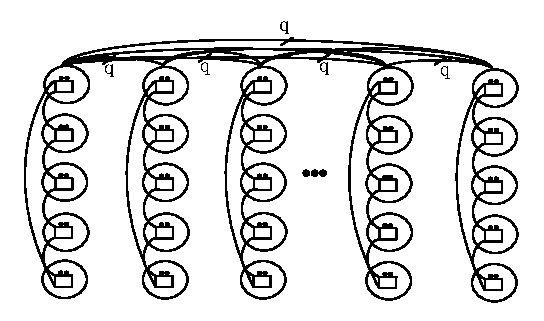
\includegraphics[width=.45\textwidth,height=.30\textwidth]{Visio-largeGF2.eps}
  \label{largeGF0}
  }
     \subfloat[GF($n,1,a,p$)]{
  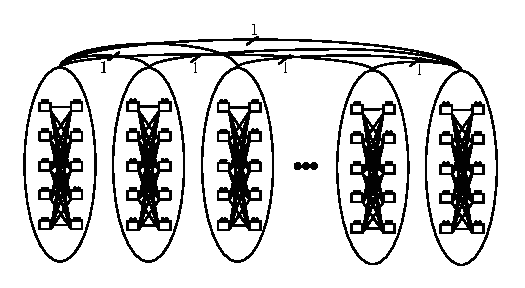
\includegraphics[width=.45\textwidth,height=.31\textwidth]{Visio-largeGF1.eps}
  \label{largeGF1}
  }

     \subfloat[GF($n,q,a,p$)]{
  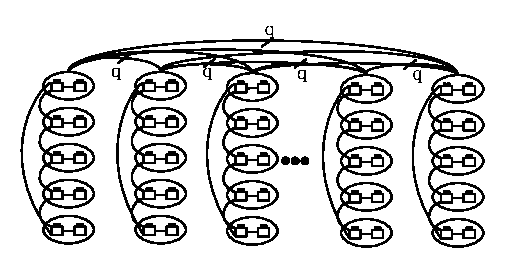
\includegraphics[width=.6\textwidth,height=.32\textwidth]{Visio-largeGF0.eps}
  \label{largeGF2}
  }
  \caption{Galaxyfly}
  \label{gfgraph}
    \end{minipage}
\end{figure}

\section{Galaxyfly结构分析}

在这一节中,我们要分析Galaxyfly结构的特征:灵活性,二分带宽,
最短路径和容错性。我们比较了我们提出的Galaxyfly(GF)和别的典型
拓扑结构,如:Dragonfly(DF)\upcite{dragonfly},Flattened Butterfly(FB)\upcite{Flattenedbutterfly}、
Fat tree(FT)和Slim Fly(SF)\upcite{slimfly}。为了方便,在下文中提到这些拓扑结构都是使用缩写。

\subsection{灵活性}

灵活性是指一个拓扑结构可以构建不同规模的网络,从P级系统到E级系统甚至更大。
这也是高效的拓扑结构必须具备的属性。我们从两个方面介绍了GF的灵活性。一种是
使用一样端口数的路由器构造不同规模的网络。另一种则是使用不同端口数的路由器
构造同一规模的网络。

图\ref{fig:Figure4}展示了不同配置下GF使用48端口的路由器能够构建出小于1K
大于10000K的网络。图中横坐标是指每个路由器连接终端的数目$p$。
在图\ref{fig:Figure3}
中,FB和FT都是三维和三层的结构。虽然DF可以调整参数$a$、$p$ 和$h$的取值来
支持不同规模的网络,但是DF的最大规模以及均衡配置是在满足$a = 2p$和$h = p$
的条件下。FB和FT的可扩展性都低于GF和DF。相比较其他拓扑结构,DF是除了GF外
可扩展性最好的拓扑结构。但是,DF仍然不能使用48端口的路由器构建100K的E级系统规模。
尽管在路由器端口数受限制的情况下,FT可以通过增加层数扩展至100K的规模。但是,这会消耗
大量路由器和缆线。在给定节点度数和网络直径,SF可以尽可能的构造更大规模。但是,SF在
路由器端口数的限制下灵活性最差,他只支持较小范围的规模。而GF能够支持不同规模的网络并
支持更大规模的网络。
\begin{figure}[t]
  \centering
  \begin{minipage}[t]{\textwidth}
   \centering
   \subfloat[GF$(n,1,1,p)$]{
  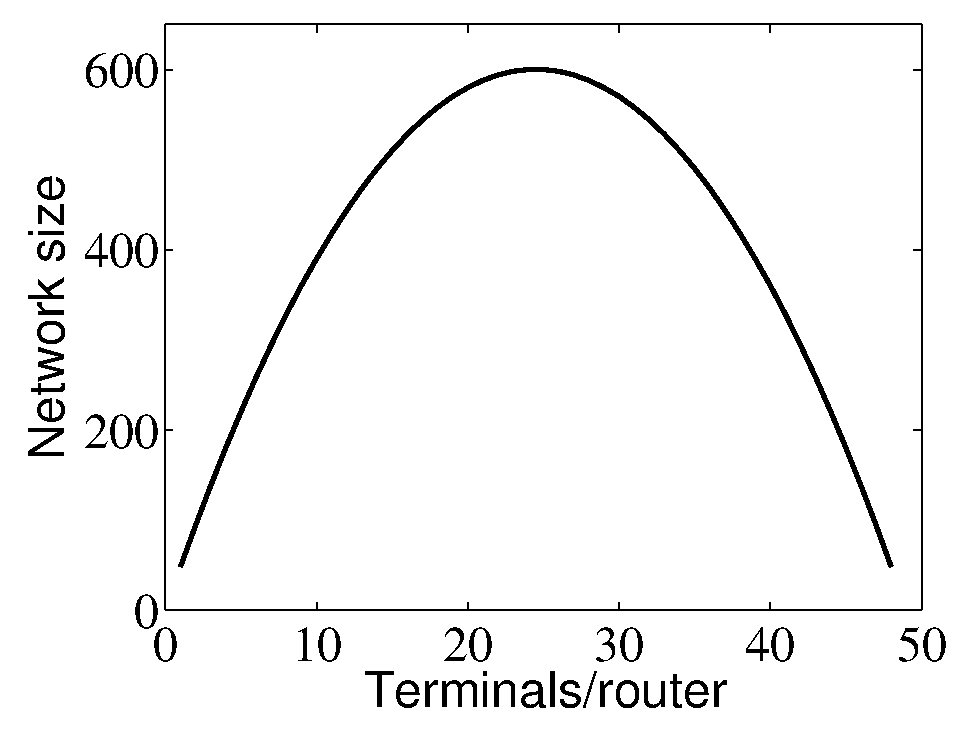
\includegraphics[width=.32\textwidth]{gf_constructibility0.eps}
   \label{fig:Figure40}
  }
     \subfloat[GF$(n,q,1,p)$]{
  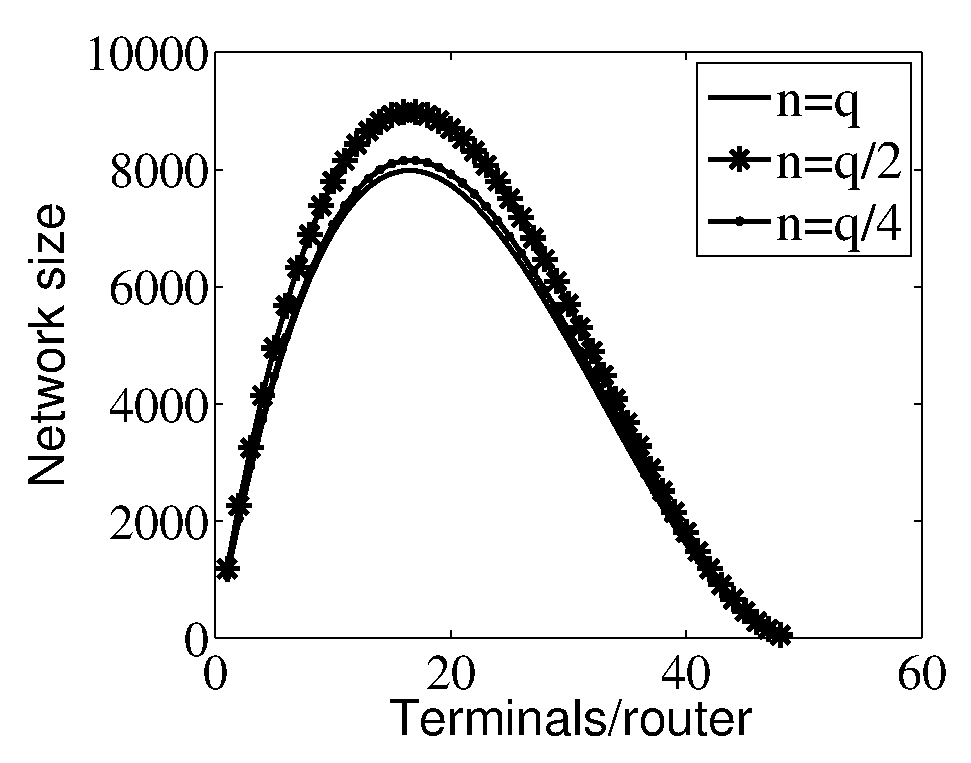
\includegraphics[width=.31\textwidth]{gf_constructibility1.eps}
   \label{fig:Figure41}
  }
     \subfloat[GF$(n,1,a,p)$]{
  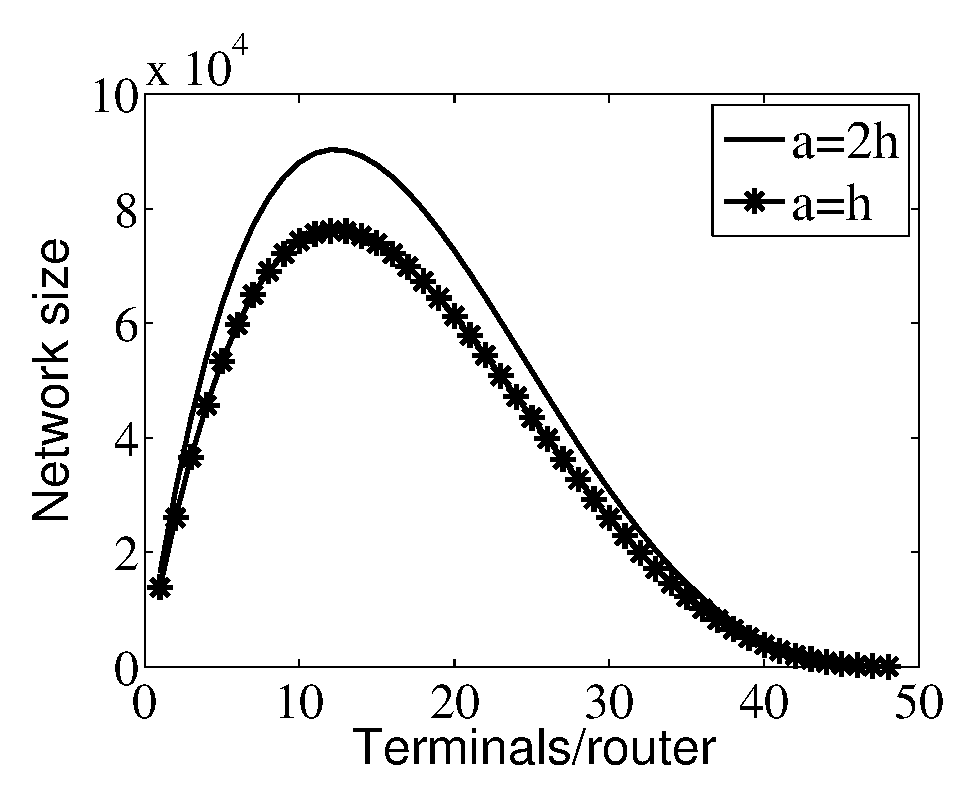
\includegraphics[width=.3\textwidth]{gf_constructibility2.eps}
 \label{fig:Figure42}
  }\\
     \subfloat[ GF$(n=q,q,a,p)$]{
  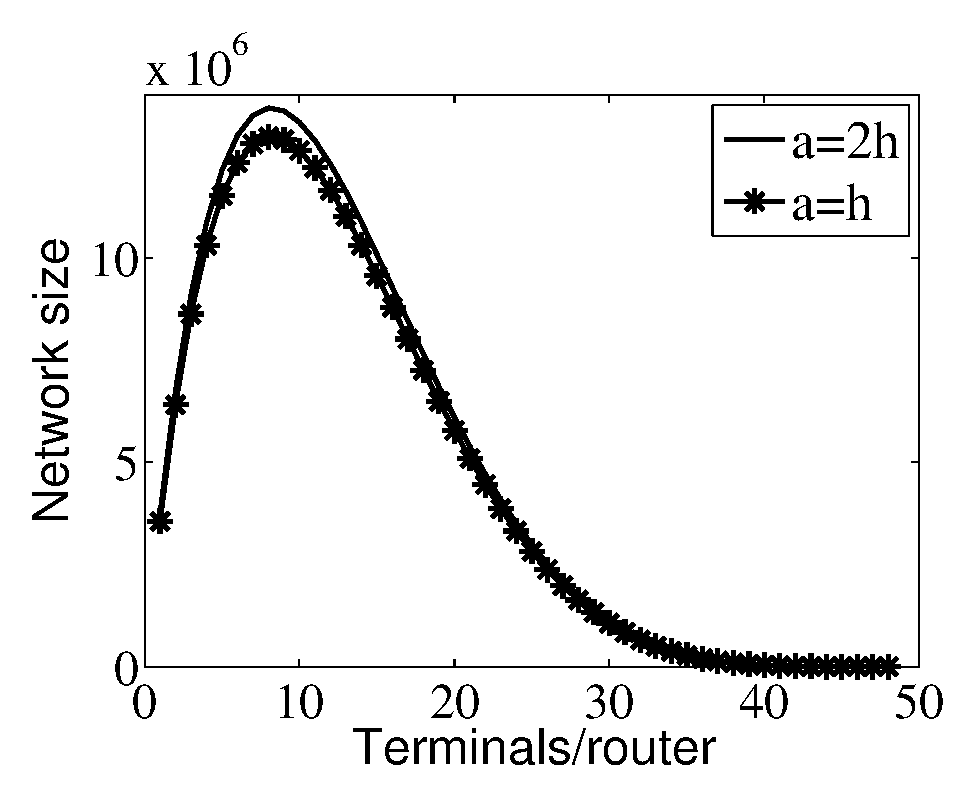
\includegraphics[width=.3\textwidth]{gf_constructibility3.eps}
 \label{fig:Figure43}
  }
     \subfloat[ GF$(n=q,q,a,p)$]{
  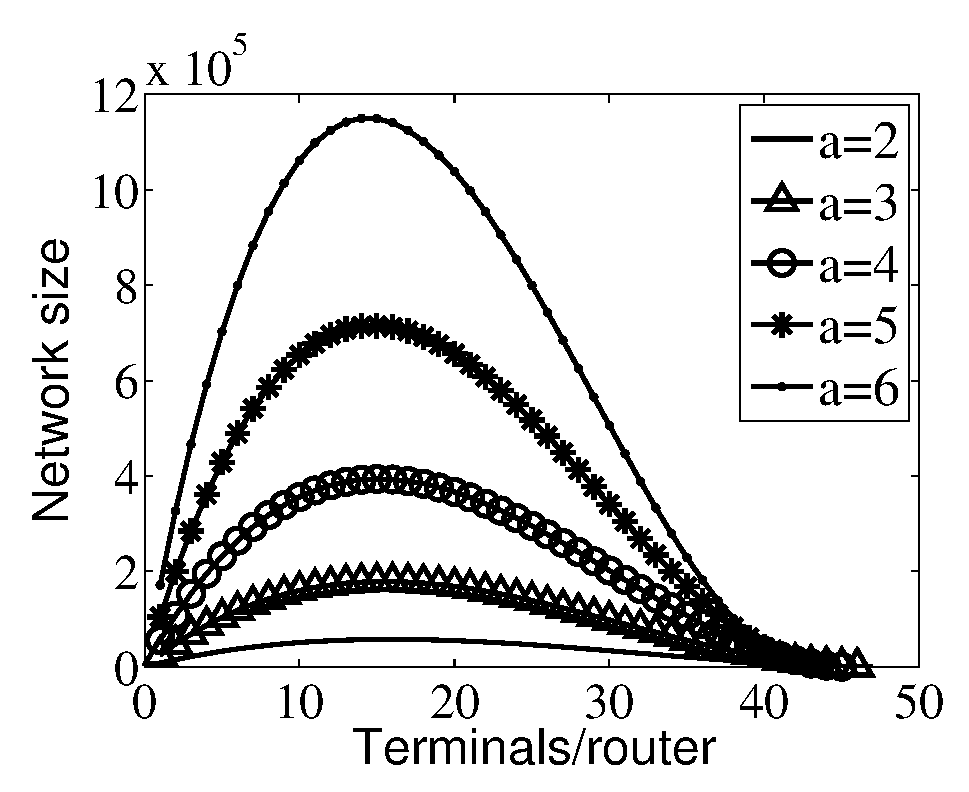
\includegraphics[width=.3\textwidth]{gf_constructibility4.eps}
   \label{fig:Figure44}
  }

   \caption{使用端口数为48路由器搭建不同配置的Galaxyfly的扩展性}
  \label{fig:Figure4}
  \end{minipage}
\end{figure}


GF$(n,1,a,p)$是DF结构,其扩展性如图\ref{fig:Figure43}所示。因此,为了
比较的公平性,我使用了DF最好的配置$a=2h$与GF比较。结果显示GF 能够
比DF最好的配置支持更大的规模。而且,GF能够配置出比DF的直径更低
的小规模系统如图\ref{fig:Figure42}所示。图\ref{fig:Figure44}
和图\ref{fig:Figure45}展现了不同的$a$值是如何影响网络规模而且
随着$a$值的增加,网络的最大规模也随之增加。通过分析GF的不同规模发现,
GF的规模越大,网络直径就越大直到上限5。因此,GF的构造实际上也是网络规模
和网络直径的权衡。

\begin{figure}[t]
  \centering
  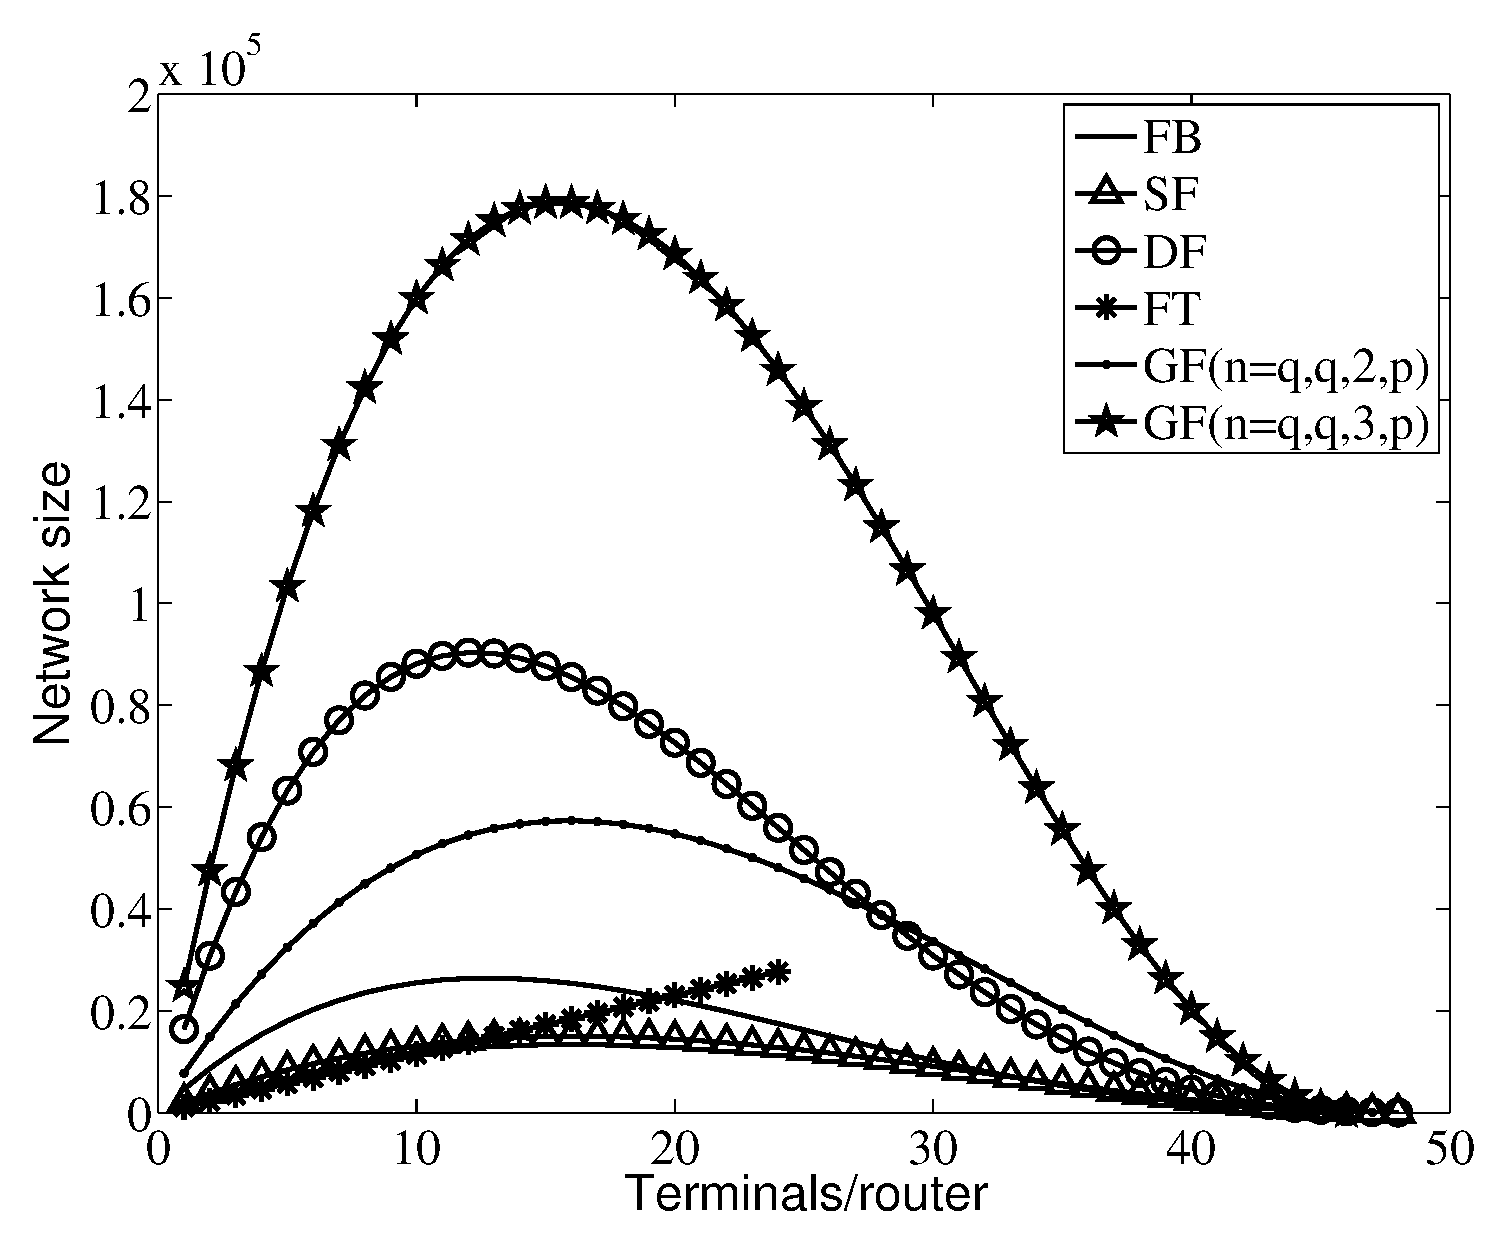
\includegraphics[width=2.5in]{difftopo_constructibility_new.eps}\\
  \caption{使用端口数为48路由器搭建不同拓扑结构的扩展性}
  \label{fig:Figure3}
\end{figure}

灵活性同时也表现在一个拓扑在同样规模下能用多少不同的路由端口数路由器构建。换句话说就是,不同的商用路由器能够被用来构造要求的网络规模。没有
对路由器的限制。特别是GF结构,同一规模能够被不同的配置使用不同范围的
端口数的路由器搭建网络。随着网络直径的增加,可构建要求规模的路由器端口数
范围越大,而且在大部分情况下支持的最小端口数则越低。

\section{可行配置}

我们考虑一个网络的可行配置决定了网络的性能。

可行配置不仅要满足路由器端口数的要求和网络规模的要求还要满足
性能的要求。GF是一个直接拓扑结构。每一个路由器的端口数$r$需要满足
$a+h+p-1\leq r$和网络规模$N$被限制在$nqap\geq N$。在给定的$r$和$N$,
这些约束提供了可行配置的范围。

二分带宽是所有网络平均二分中最小切割的带宽,是评价拓扑结构传统的
指标。为了公平的比较我们的设计和已有的拓扑结构,我们利用二分带宽来
分析拓扑结构的静态性能。由于GF 和SF的不规则性,计算分析这两种拓扑结构的
二分带宽不能简单用公式表示。但是,我们可以使用图划分的工具METIS\upcite{METIS}近似求解GF和SF拓扑结构的二分带宽。每个非堵塞拓扑结构
至少有$N/2$条双向链路通过每个图的二分最小切割。在均衡随机通信负载下,
只要图的二分最小切割有$N/4$条双向链路就使网络是均衡负载的。我们
假设每条链路的带宽为1,那么网络的最小二分切割就是二分带宽。因此,
$\beta=(C_{min}/(N/2))$描述的就是拓扑结构的二分带宽。一般情况下,
拓扑结构的二分带宽大于等于要求的二分带宽。

我们的目标是找到可行的配置满足上述限制。图\ref{fig:Figure6} 展示了路由端口数$r\leq 48$ (当前商用高阶路由器端口数)以及$\beta \approx 0.5$。在不同的
网络直径情况下,我们可以构造出不同规模的GF。有5个参数影响GF 的设计空间。
一旦$n$,$q$和$a$确定,那么$h$ 就是常数。另外,如果$h$,$q$和$a$确定或者
$n$,$h$和$a$确定,则$n$或者$q$是常数。


 \begin{figure}[t]
  \centering
  \begin{minipage}[t]{\textwidth}
   \centering
  \subfloat[GF$(n,q,1,p)$]{
  \includegraphics[width=.31\textwidth]{BB_1_v11.eps}
  \label{BB_1_v11}
  }
    \subfloat[GF$(n,1,a,p)$]{
  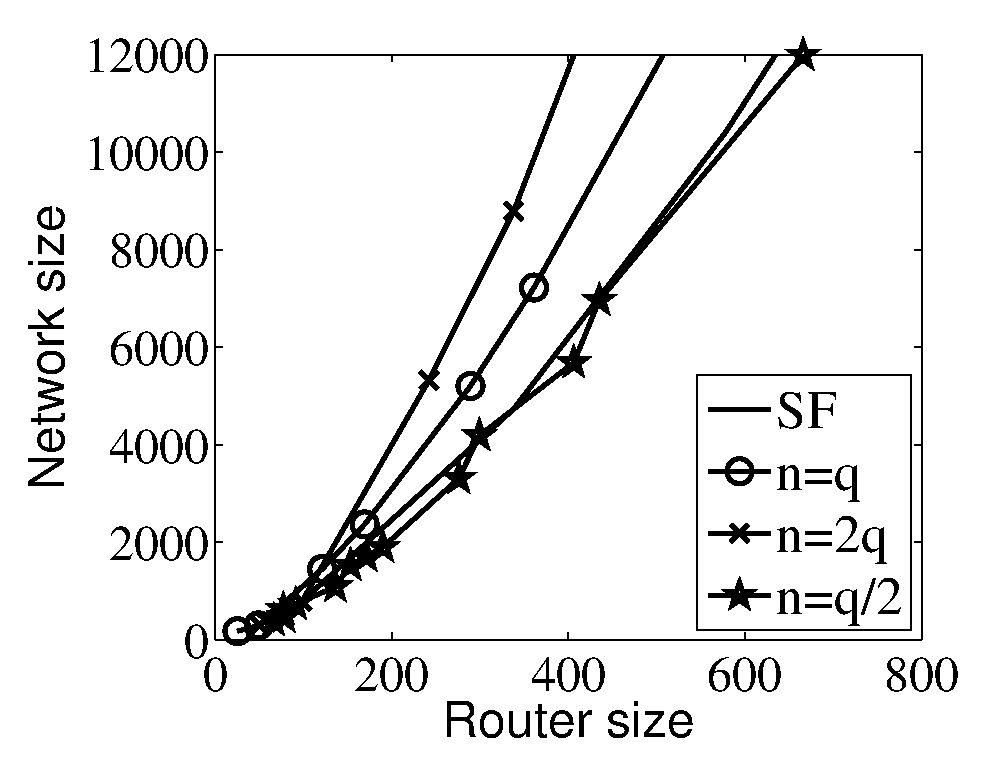
\includegraphics[width=.31\textwidth]{BB_1_v12.eps}
  \label{BB_1_v12}
  }
    \subfloat[GF$(n=q,q,a,p)$]{
  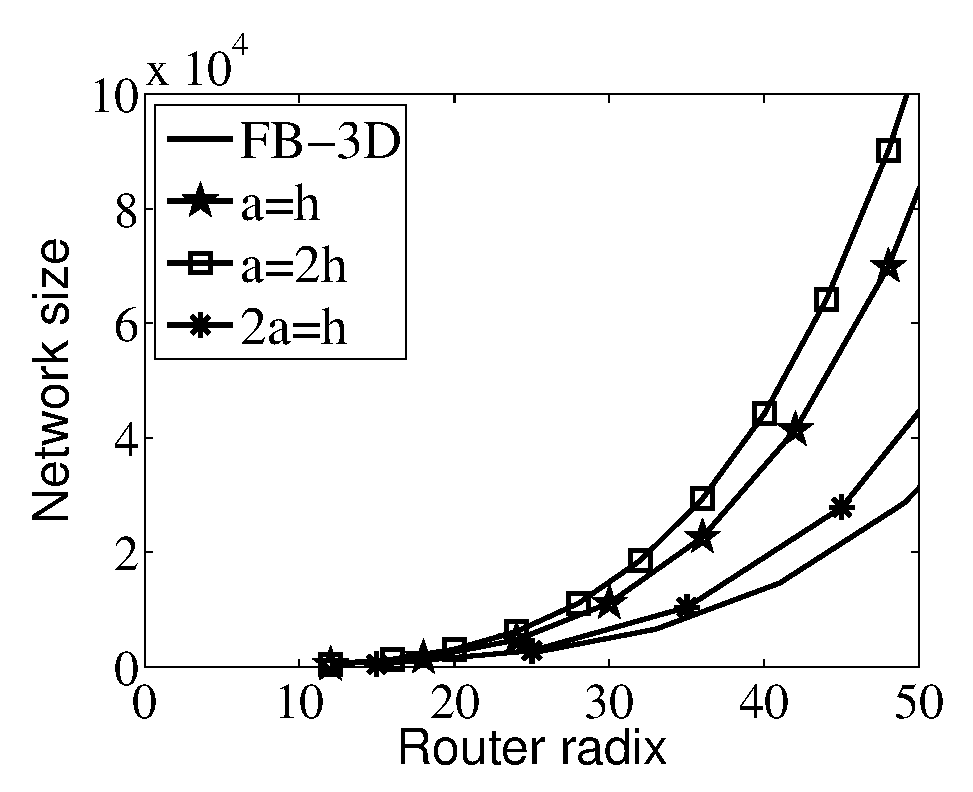
\includegraphics[width=.3\textwidth]{BB_1_v13.eps}
  \label{BB_1_v13}
  }
  \\
    \subfloat[GF$(n,q,1,p)$]{
  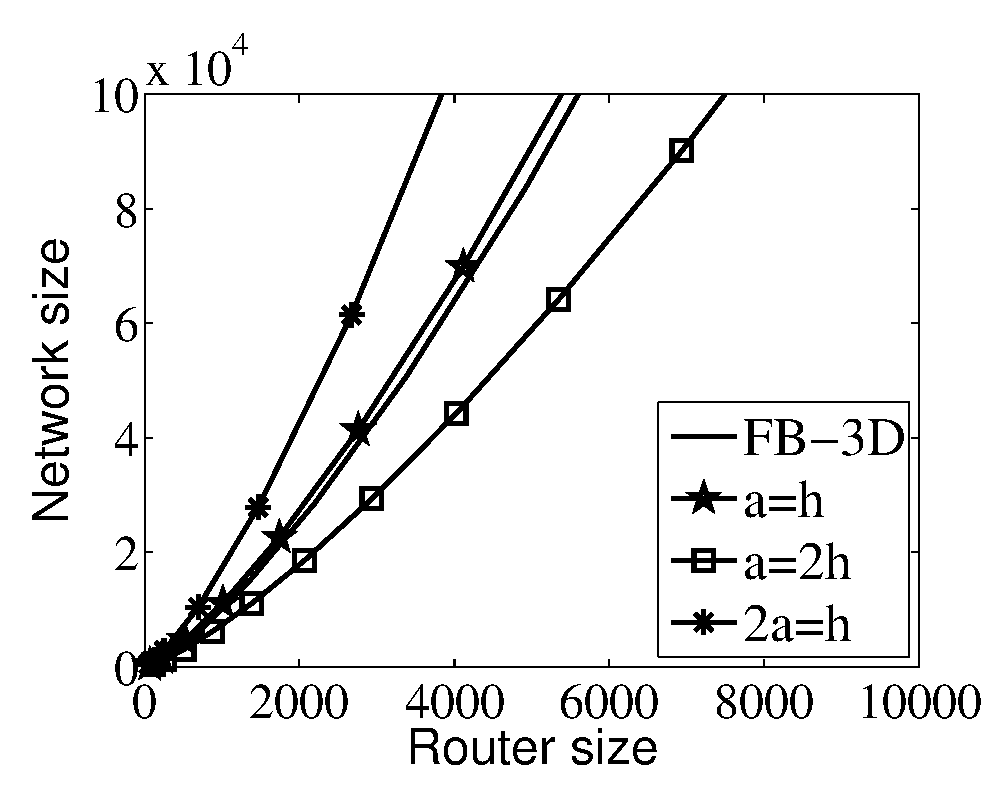
\includegraphics[width=.315\textwidth]{BB_1_v14.eps}
  \label{BB_1_v14}
  }
    \subfloat[ GF$(n,1,a,p)$]{
  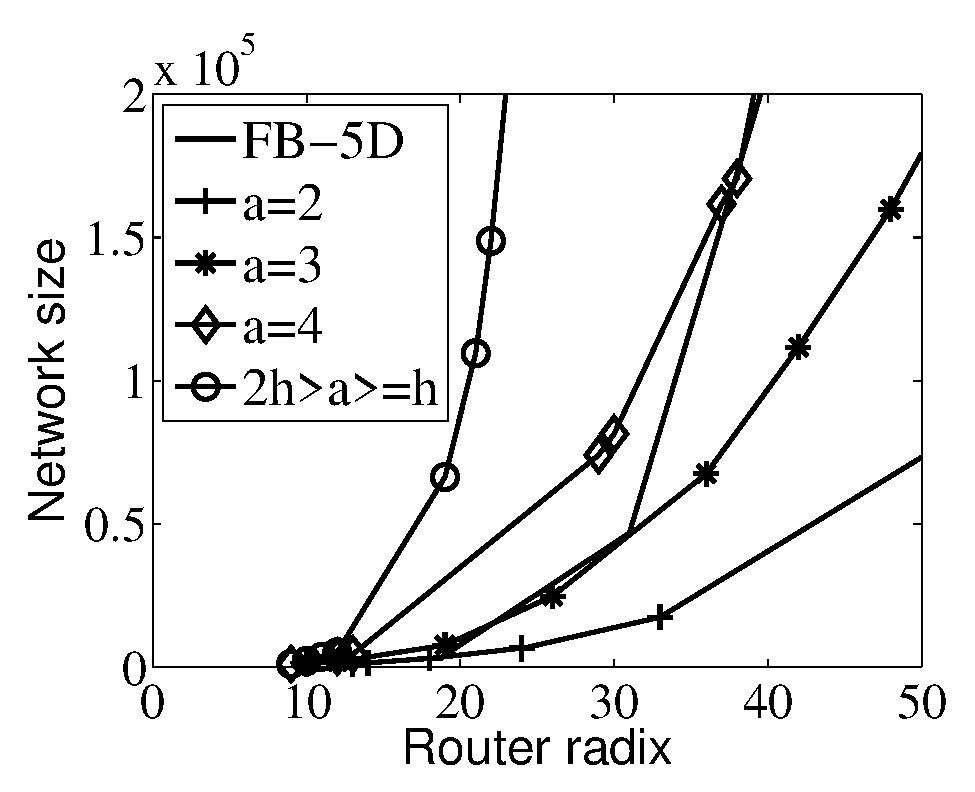
\includegraphics[width=.31\textwidth]{BB_1_v15.eps}
  \label{BB_1_v15}
  }
    \subfloat[GF$(n=q,q,a,p)$]{
  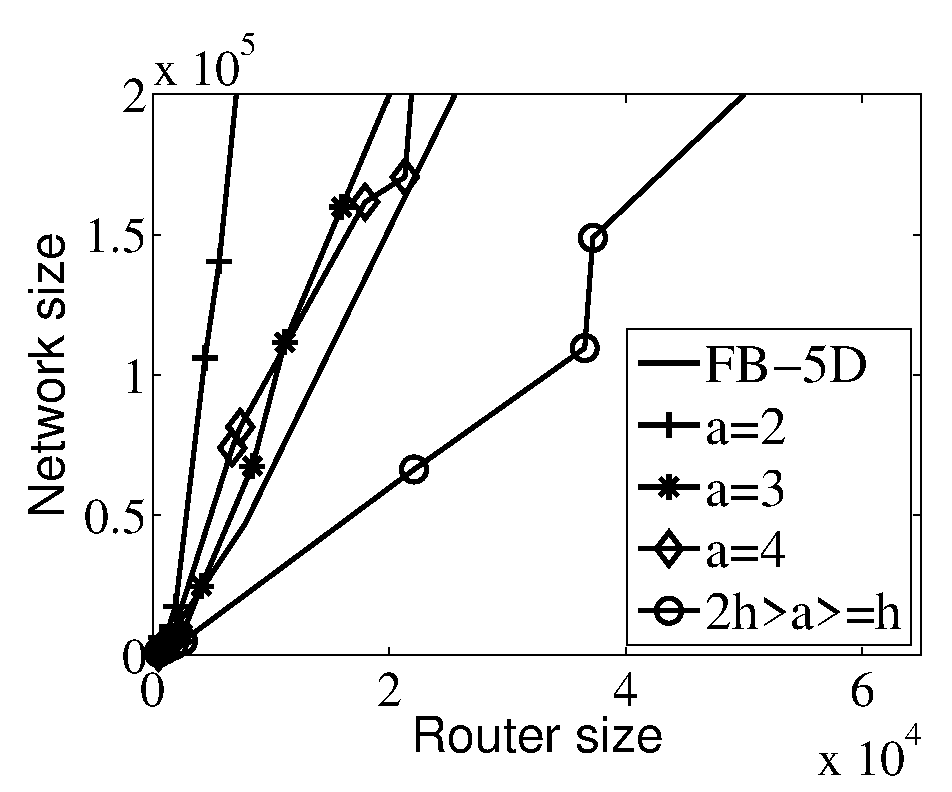
\includegraphics[width=.3\textwidth]{BB_1_v16.eps}
  \label{BB_1_v16}
  }
  \caption{不同配置下的Galaxyfly和其他拓扑结构在全局二分带宽率为0.5的设计 范围:路由器端口数和网络规模的关系:(a)--(c); 路由器规模和网络规模:(d)--(f)。 }
  \label{fig:Figure6}
  \end{minipage}
\end{figure}

图\ref{BB_1_v11}、图\ref{BB_1_v12}和图\ref{BB_1_v13}
描述了随着端口数$r$增加,网络规模$N$的趋势。相应地,
图\ref{BB_1_v14}、图\ref{BB_1_v15}和图\ref{BB_1_v16}
描述了随着网络规模$N$的增加,路由器数量的增长趋势$N_r$。对于GF$(n,q,1,p)$,我们选择了不同的$n$和$q$配比关系去分析网络规模的趋势
如图\ref{BB_1_v11}所示。使用同样的路由器端口数$r$,我们能使用
SF构造更大规模。但是,在同一规模下,GF$(n=q,q,1,p)$和GF$(n=2q,q,1,p)$
可以用比SF更少的路由器数量搭建网络。GF$(n,1,a,p)$是灵活的DF 结构。那么,
当$a=2h$即$n=a^{2}/2+1$时,GF$(n,1,a,p)$是均衡的DF而且是最大规模
的配置,比3维FB结构的扩展好,如图\ref{fig:Figure6}b所示。但是,在使用
端口数为48的路由器时,最大规模仍然不能达到100K。5维的FB、GF$(n=q,q,4,p)$
和GF$(n=q,q,2h>a\geq h,p)$在使用48端口的路由器时可以构造100K 规模的网络,
如图\ref{BB_1_v13}和图\ref{BB_1_v16}所示。GF$(n=q,q,2h>a\geq h,p)$相比别的配置和5维FB,消耗更多的路由器,但是,GF$(n=q,q,2h>a\geq h,p)$使用的路由器的端口数是最小的。在网络规模为200K 时,
GF$(n=q,q,2h>a\geq h,p)$的路由器端口数只有5维FB的一半。



我们也分析了不同$\beta$限制下,路由器数量和网络规模的关系。
当$\beta$的值越高,则需要更多的路由搭建同一规模的网络。
我们使用一样的参数$a$,$h$和$p$并满足$a=2h=2p$的条件去构造DF和GF,
GF的规模可以达到将近$a^2/4$倍DF的规模。但是,GF的二分带宽只是
稍微低于DF的二分带宽。因此,我们可以使用同样的路由器构造
更大规模的GF。在表\ref{Table5} 中,我们给出了一些GF和DF在同样
$a$,$h$和$p$参数下的示例。GF 是一个灵活的拓扑结构而且能够找到一些
满足网络构建限制的配置。这是灵活的权衡二分带宽、网络规模、路由器规模
以及路由器端口数去构造GF。

\begin{table}[t]
\caption{同样参数配置$a$、$h$和$p$的Galaxyfly和Dragonfly的二分带宽}
\centering
\begin{tabular}{c| c| c| c |c}\hline
  \centering
  Topology	& GF$(n,q,a,p)$ & $N_r$	& \tabincell{c}{Bisection \\ Bandwidth}	& $\beta$	\\\hline
  \multirow{5}*{DF}
  &$(9,1,4,2)$	&36	&20	&0.56 \\\cline{2-5}
  &$(19,1,6,3)$	&114	&94	&0.55 \\\cline{2-5}
  &$(33,1,8,4)$	&264	&275	&0.52 \\\cline{2-5}
  &$(55,1,10,5)$	&550	&701	&0.51 \\\cline{2-5}
  &$(73,1,12,6)$	&876	&1332	&0.51 \\\hline
  \multirow{5}*{GF}
  &$(5,7,4,2)$	&140	&44	&0.31	\\\cline{2-5}
  &$(9,19,6,3)$	&1026	&560	&0.36 \\\cline{2-5}
  &$(17,31,8,4)$	&4216	&2350	&0.28 \\\cline{2-5}
  &$(30,53,10,5)$	&15900	&14026	&0.35 \\\cline{2-5}
  &$(37,73,12,6)$	&32412	&36676	&0.38 \\\hline
\end{tabular}
 \label{Table5}
\end{table}

二分带宽是一个理论指标和是网络划分两部分之间路由的带宽上限。
在给定的不同通信模式下和不同路由算法,有效地二分带宽小于
理论的二分带宽\upcite{multistage}。另外,在GF的本地单元
采用的全互连图中,二分带宽为$a^2/4$。如果超级节点不堵塞,
那么要求在均衡随机通信模式下,至少需要$ap/2$条双向链路。
如果我们设计一个可行的GF配置,这个也不得不考虑超级节点内的
参数配置。

\subsection{最短路径}

最短路径数量是一个负载均衡的网络重要的指标。表\ref{Tablesp} 中
分析了不同配置的GF和SF的最短路径数量。$SP$是指最短路径数量大于1
的节点对数量与网络中所有节点对(即$N_r\times (N_r-1)$)的比值。
集群内的$SP$是指集群内最短路径大于1的节点对数量与网络中所有节点对
的比值。相反,集群间的$SP$是指集群间最短路径大于1的节点对数量与网络中所有节点对的比值。对于SF,尽管在给定路由器端口数可以构造更大的直径为2的
拓扑,但是最短路径数量却远远小于其他拓扑结构,如表\ref{Tablesp}所示。
GF$(n,q,1,p)$也是一个直径为2的拓扑结构,但是他的$SP$却大于SF。实际上这是
做了路由器端口数和$SP$的权衡。GF$(n,q,1,p)$链路数多于SF。GF$(n,1,a,p)$
是DF结构,以及他的$SP$值接近GF$(n,q,1,p)$的$SP$。GF$(n,q,a,p)$的$SP$
最高而且使用的路由器端口数最少,但是他的网络直径是5。绝大多数集群内
$SP$是低于集群间$SP$的,因为$q$的取值。因此,为了增强网络的负载均衡,
可以充分利用集群间的最短路径数量。

\begin{table}[t]
\caption{最短路径数量}
\centering
\begin{tabular}{c| c| c |c|c|c}\hline
  \centering
  拓扑结构 & $k'$ & $N_r$ & $SP$ & 集群内$SP$ & 集群间$SP$\\\hline
  \multirow{2}*{SF}
  &25		&578	 &0.01 &0.01 & 0 \\\cline{2-6}
  &35		&1058	 &0.05 &0.01 & 0.04\\\hline

   \multirow{2}*{GF(n,q,1,p)}
  &31		&496	&0.14 &0.03 &0.11\\\cline{2-6}
  &47		&992	&0.13 &0.01 &0.12\\\hline

   \multirow{2}*{GF(n,1,a,p)}
  &14		&510	&0.17 &0 &0.17\\\cline{2-6}
  &17		&876	&0.15 &0 &0.15\\\hline

   \multirow{2}*{GF(n,q,a,p)}
  &8		&510	&0.43 &0.03 &0.41\\\cline{2-6}
  &8		&966	&0.51 &0.06 &0.44\\\hline
\end{tabular}
\label{Tablesp}
\end{table}

\subsection{容错性}

我们通过模拟随机链路的出错性来分析拓扑结构的容错性
以及结果反映在平均路径的长度和网络直径。不同程度
的随机链路出错直到网络不连通。图\ref{fig:Figure8}
展示了不同配置的GF和其他拓扑结构随着链路出错率的
增加平均最短路径合网络直径的变化。对于GF、DF和SF,
容错性随着路由器规模的增加而提升。图\ref{nr1}
和图\ref{nr2}展示了GF$(n,q,1,p)$和SF在路由器
规模0.2K-2K下容错性的变化。图\ref{nr3}
和图\ref{nr4}展示了GF$(n,q,a!=1,p)$和DF在路由器
规模0.2K-2K下容错性的变化。在路由器规模为2K的情况下,
GF$(n,q,1,p)$的链路出错率可以增加到$90\%$,而SF可以
增加到$86\%$。GF$(n,q,a!=1,p)$ 和DF只能分别允许$60\%$和
$65\%$的链路出错。GF$(n,q,1,p)$和SF的容错性能比GF$(n,q,a!=1,p)$
和DF在同一规模下容错性好是因为更短的网络直径和更多的链路。


\begin{figure}[t]
  \centering
  \begin{minipage}[t]{\textwidth}
   \centering
  \subfloat[]{
  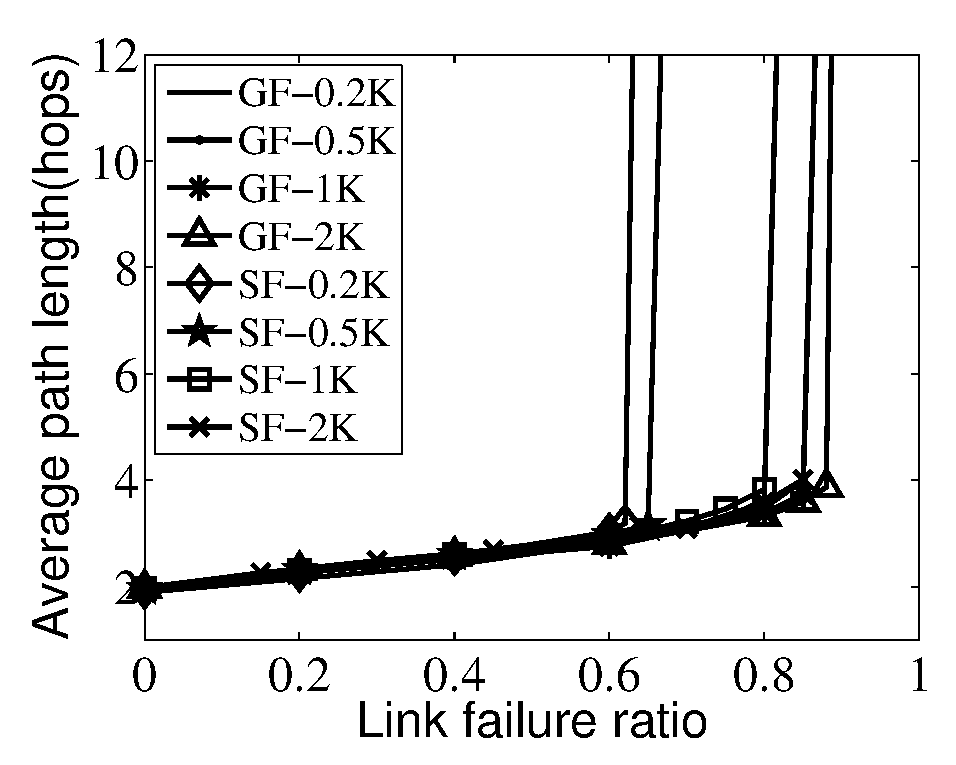
\includegraphics[width=.4\textwidth]{nr1.eps}
  \label{nr1}
  }
   \subfloat[]{
  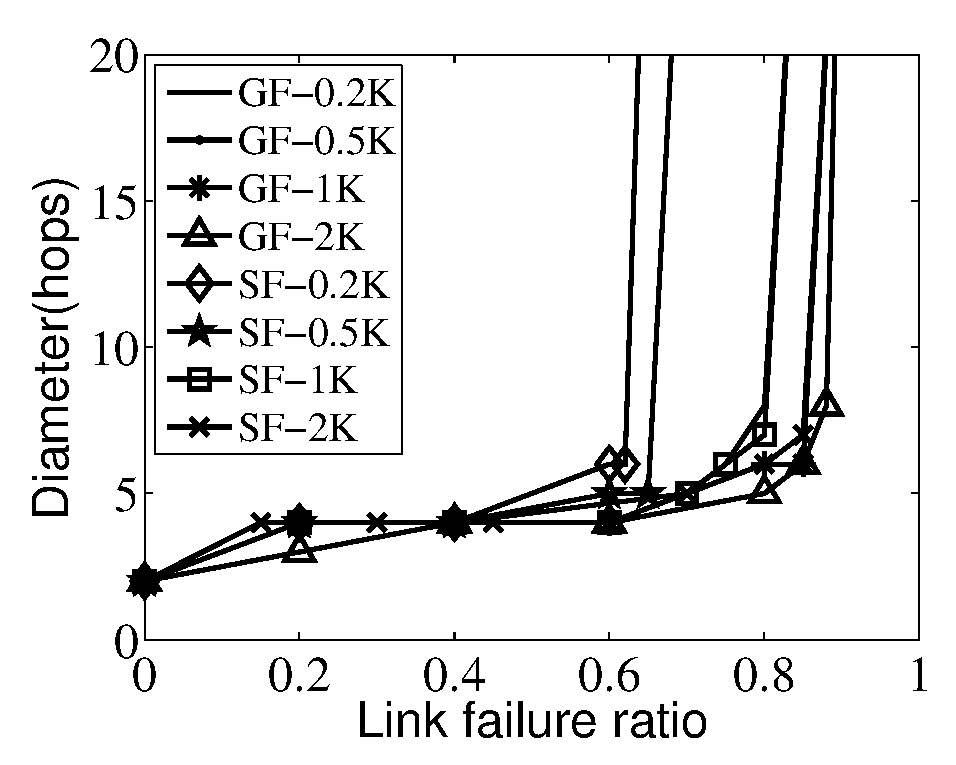
\includegraphics[width=.4\textwidth]{nr2.eps}
  \label{nr2}
  }\\
   \subfloat[]{
  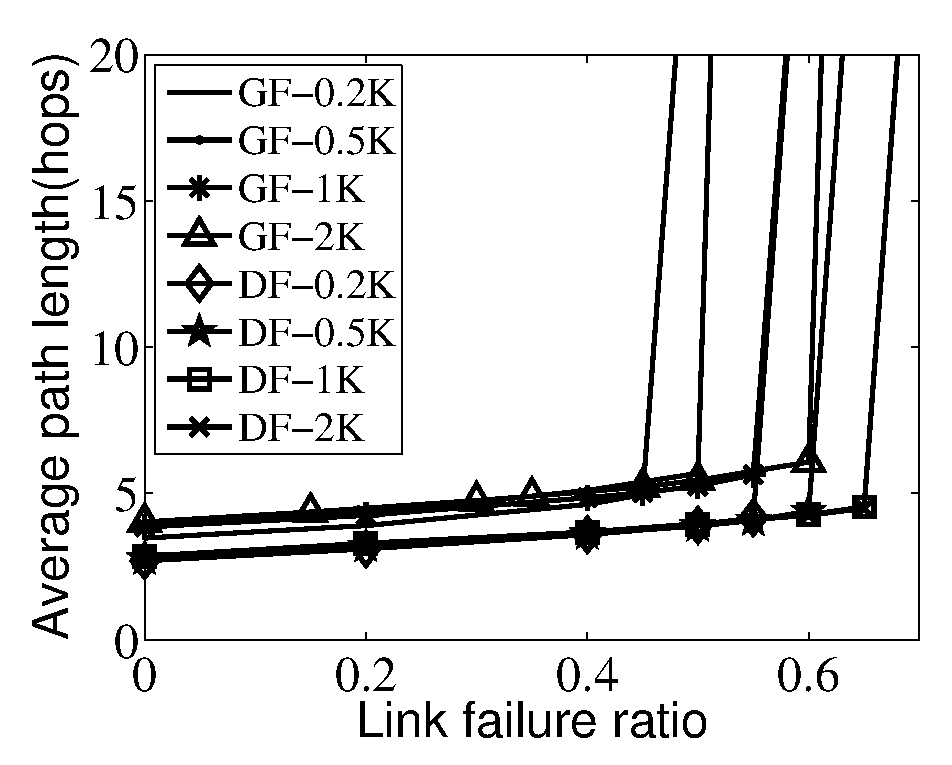
\includegraphics[width=.4\textwidth]{nr3.eps}
  \label{nr3}
  }
   \subfloat[]{
  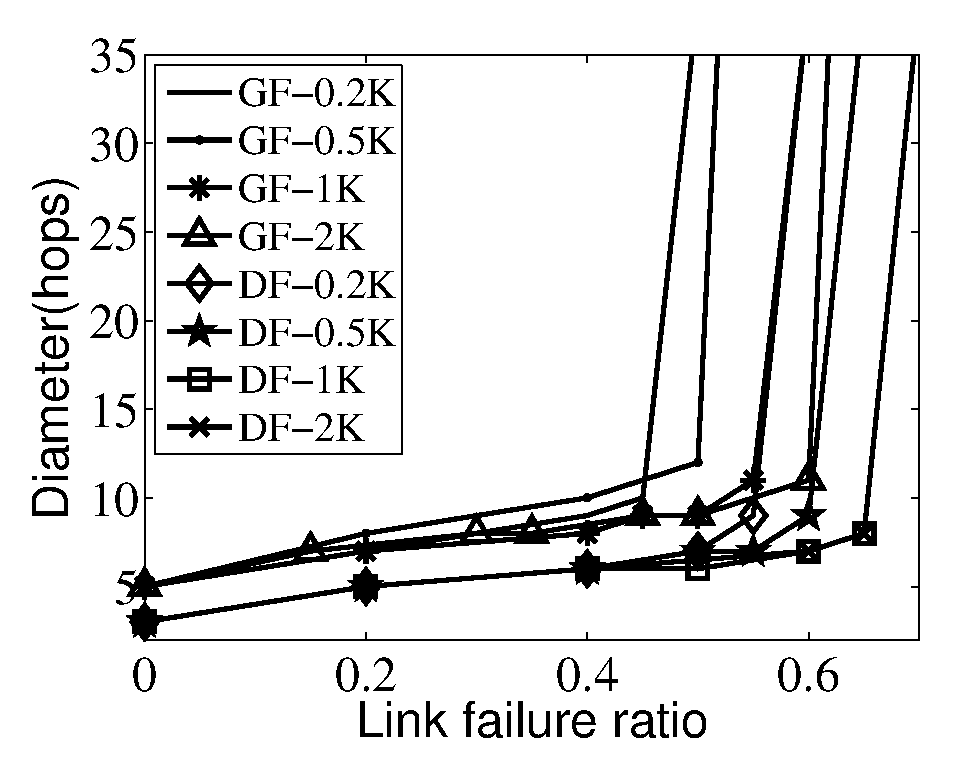
\includegraphics[width=.4\textwidth]{nr4.eps}
  \label{nr4}
  }
  \caption{ 不同链路错误率下GF$(n,q,1,p)$和Slim Fly平均最短路径长度和网络直径的变化(a)--(b);GF$(n,q,a\neq1,p)$和Dragonfly平均最短路径长度和网络直径的变化 (c)--(d)。}
  \label{fig:Figure8}
   \end{minipage}
\end{figure}


\section{路由算法}

在这一节中将给出Galaxyfly结构的最短路径路由和非最短自适应路由算法
以及介绍路由算法配套的死锁避免机制。报文从源节点直接传输给直接相连
的源路由节点$R_s$并由此转发路由至目的节点直接相连的目的路由节点
$R_d$。

\subsection{最短路径路由算法}

Galxyfly的最短路径路由算法(MIN)将要分两种情况讨论:
一是针对GF$(n,q,1,p)$配置;第二种则是针对GF$(n,q,a\neq 1,p)$配置。

在GF$(n,q,1,p)$的情况下,GF是一个直径为2的拓扑结构。所以,
一个报文被传输要么直接1跳($R_s$直接连接$R_d$)或者路由经过2跳
($R_s$通过中介节点$R_i$连接$R_d$)。

GF$(n,q,a\neq 1,p)$的MIN取决于源超级节点$G_s$
和目的超级节点$G_d$的连接关系。路径长度最多5跳。具体路由执行
如下面讨论所示:

步骤1:如果$G_s\neq G_d$而且$G_s$和$G_d$不相连,那么就要找一个公共
相邻超级节点$G_i$作为中介超级节点。那么报文通过$G_s$的$R_a$
将要先到达中介超级节点
$G_i$的路由节点$R_x$。继续第二步。

如果$G_s\neq G_d$但是$G_s$和$G_d$有一条链路相连,那么报文要么
通过$R_s$的链路或者通过$G_s$超级节点中的其他路由节点$R_a$
到达$R_d$。接着,报文到达$G_d$ 的路由节点$R_b$。继续第三步。

步骤2:如果没有直接链路从$R_x$ 到达超级节点$G_d$,那么,通过
超级节点$G_i$中的其他路由节点$R_y$使报文到达目的超级节点
$G_d$的$R_b$。继续第三步。

步骤3:如果$R_b \neq R_d$,那么在同一个超级节点$G_d$内要
经过一条本地链路,那么报文将要到达$R_d$。

针对Galaxyfly结构,对MIN可以做一个小优化。
根据超级节点$G_s$和$G_d$的位置,MIN可以调整
集群内的路由使得路由负载均衡通过多条最短路径
如表\ref{Tablesp}所示。
如果$G_s$和$G_d$在同一个集群内而且不相连,
那么$G_s$和$G_d$之间至少存在一个公共相
邻超级节点。因为在$q$模4余1的情况下,
每个集群超级节点组成的结构是一个强正则图。
例如,如果$q=5$,那么同一个集群内不相连
的超级节点之间至少有一个公共相邻超级节点。
如果$q=13$,那么同一个集群内
两个不相连的超级节点之间有
3个公共相邻超级节点。那么,在$G_s$和
$G_d$之间有不同的路径可以选择,路由可以随机
选其中一条。但是,$G_s$和
$G_d$之间有多条最短路径,不代表$R_s$和
$R_d$之间有多条最短路径,还要根据$R_s$和
$R_d$的超级节点之间
的连接与公共相邻超级节点的位置关系选择最短的路径。如果采用的路由表路由报文,那么我们
可以通过选择集群间的多条最短路径来提高网络的
负载均衡,如表\ref{Tablesp}所示。

\subsection{非最短路径自适应路由算法}

对于非最短自适应路由算法,我们根据当前路由器的缓冲区
状态来选择最短路径路由或是非最短路径路由。对于Galaxyfly
结构,不同的配置可以使得网络的直径从2到5。因此,为了控制
两个终端的之间的跳步数和减少虚拟通道(VC)的数量,非最短
自适应路径采用了限制随机选择路径的长度,使得最长路径
分别在5跳、6跳或者7跳以内。我们设计了三种路由算法:
非最短自适应随机链路路由算法(NAR)、非最短自适应本地
链路路由算法(NAL)以及非最短自适应全局链路路由算法(NAG),
他们都是基于Galaxyfly结构特性、非最短路径路由算法以及全局
自适应负载均衡路由算法设计的\upcite{Singh}\upcite{slimfly}\upcite{dragonfly}。

NAR是一个非最短自适应路由算法。为了限制路径长度,
NAR只在两个终端在同一个集群内但是分别在两个相连的超级节点
内才会执行非最短路径路由。因为,两个超级节点之间
可能存在多个公共相邻超级节点。NAL则是允许在源超级节点
内多绕行1跳。NAG则是允许绕行到别的超级节点。因此,对NAL以及
NAR的限制分别为6跳和7跳。NAG的最长路径通过3跳超级节点间链路
和4跳超级节点内的链路。在NAL和NAR中,选择非最短路径和最短路径
都是发生在源路由节点。根据缓冲区队列的占有率来判断走哪一条路。
$Q_{min}$是最短路径端口的缓冲区队列的占有率。$Q_{nonmin}$是非
最短路径端口的缓冲区队列的占有率。$Th_{min}$和$Th_{nonmin}$ 则
分别是选择走最短路径和非最短路径的阈值。如果$Q_{nonmin}<Th_{nonmin}$而且
$Q_{min}>Th_{min}$,那么报文将要选择非最短路径。 $Th_{nonmin}$ 和 $Th_{min}$ 都是通过多次模拟得到的经验值。我们设置
$Th_{nonmin}=0.5\times Q_{min}$ 和 $Th_{min}=0.8\times$ $缓冲区容量$。

\subsection{死锁避免机制}

Galaxyfly的死锁避免机制与Dragonfly\upcite{dragonfly}和Slim Fly\upcite{slimfly}的死锁避免机制类似。基于距离的死锁避免机制
每一跳都切换一条VC,因此,需要有最长路径跳步数一样的VC数来
避免死锁。报文开始注入时使用编号为0的VC,每经过一跳使用的VC
编号加一\upcite{Prevention}\upcite{Rlmolm}。 报文在最后一条VC的时候
不会被堵塞是因为报文要被吸收。因此,报文要么前进走更高编号的VC
要么就是要被终端吸收。在Galaxyfly结构中,我们使用递增的方法使用
VC。由于Galaxyfly划分了超级节点,我们能复用本地端口的VC
和全局端口的VC并减少VC的数量。图\ref{fig:Figure9}中介绍了不同配置
的Galaxyfly的无死锁路由算法是如何使用VC的。例如,在图\ref{fig:Figure93}
中,报文最多经过3条本地链路和2 条全局链路。因此,在MIN中要求至少3条本地链路VC和2条全局链路VC来避免出现环。

相似的,NAR、NAL以及NAG算法分别需要3、4、4条本地链路VC和2、2、3条全局链路
VC。另外,我们也能采用逃逸网络或者转弯模型替代VC去消除链路依赖
\upcite{Rlmolm}\upcite{OFAR-CM}\upcite{On-the-Fly}。

\begin{figure}[t]
  \centering
   \begin{minipage}[t]{\textwidth}
   \centering
  \subfloat[diameter = 2]{
  \includegraphics[width=.25\textwidth]{Visiomind1.eps}
  \label{fig:Figure91}
  }
   \subfloat[diameter = 3]{
  \includegraphics[width=.5\textwidth]{Visiomind2.eps}
  \label{fig:Figure92}
  }
  \\
    \subfloat[diameter = 5]{
  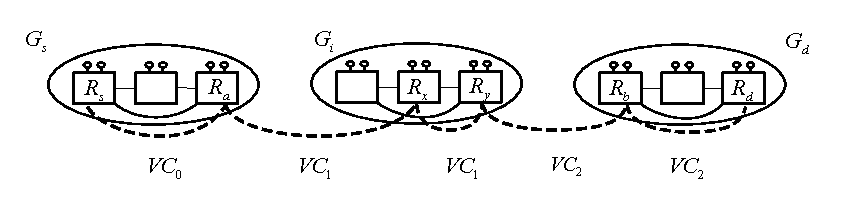
\includegraphics[width=.75\textwidth]{Visiomind3.eps}
  \label{fig:Figure93}
  }
  \caption{Galaxyfly的最短路径路由算法}
  \label{fig:Figure9}
  \end{minipage}
\end{figure}

\section{性能分析}

在这一章节中,我们使用一个时钟精确的网络模拟器Booksim\upcite{Booksim}模拟Galaxyfly(GF)
和其他拓扑结构并且通过一个伯努力分布报文注入模型分析不同
拓扑结构的性能。首先,我们在几种典型的通信模式下评测了不同配置下的GF,并分析了在
不同的报文长度及不同路由算法下的性能。第二,我们比较了GF和其他高阶拓扑结构
在不同的通信模式下的性能。
第三,我们提出了一个物理布局并评测了不同拓扑结构在这种物理布局下性的性能。
最后我们设计了一种新的混合通信模式评测GF和其他高阶拓扑结构的性能。

\textbf{路由器:}我们使用了传统的具备完整的路由器流水线的输入队列(input-queue (IQ))路由器模型。
路由器是基于Virtual Cut-through(VCT)交换机
制。我们假设信用处理过程需要2 个时钟周期,路由计算模块需要2 个时钟周期,以及交换分配模块,
虚通道(VC)分配模块和crossbar 处理模块都需要1个时钟周期。crossbar的输入和输出的加速比都是1。
内部传输数据链路数率是链路传输速率的两倍。

\textbf{网络:} 默认情况下,链路传输延迟为1个时钟周期以及报文长度为1个切片大小。
我们提供了两种链路传输延迟的配置。一种是每一条链路的传输延迟都是1个时钟周期。
根据这种配置,我们可以减少不同拓扑结构在构造同等规模的网络时使用不同端口数的路由器而造成的影响并观察网络状态。在\upcite{slimfly}
和\upcite{dragonfly}中,链路传输延迟也是设置为1个时钟周期。另外一种配置是为
了模拟实际系统物理布局而根据物理布局中的位置设置延迟。机柜间链路包括路由
器流水线的延迟一共100个周期,而机柜内链路则是50个周期。
每个端口的缓冲区容量是256个切片。缓冲区的管理机制采用每个VC 拥有
5个切片的私有存储空间,其他的缓冲区由所有VC共享。我们比较的拓扑结构
在均衡随机通信负载下的全局带宽至少$N/4$条双向链路经过任意切割以及
二分带宽率$\beta$都大于0.5
网络的规模约为$N\approx 3K$以及不同的拓扑结构在规模上的差别控制在10\%以内。
我们比较了不同的Galaxyfly结构的不同配置,如表\ref{fig:Figure6}所示。其他拓扑结构
的配置也如表\ref{Table6}所示。
Fat tree(FT)是高性能计算系统和数据中心系统最常用的拓扑结构之一。
Flattened Butterfly(FB)和Dragonfly(DF)是高阶互连网络的典型拓扑结构。
Slim Fly(SF)则是最新提出的低直径高性能互连网络。


\begin{table}[t]
\caption{拓扑结构配置}
\centering
\begin{tabular}{c| c| c|c| c |c}\hline
  \centering
  Topology	& $r$ &$p$ &Diameter & $N_r$ 	& $\beta$	\\\hline
  GF$(11,29,1,10)$ &34 &10 &2	&319 		&0.60	\\\hline
  GF$(15,29,1,7)$ &35 &7 &2	&435 		&1.12 \\\hline
  GF$(56,1,11,5)$ &20 &5 &3	&616 		&0.51 \\\hline
  GF$(81,1,10,4)$ &21 &4 &3	&810 	&1.01 \\\hline
  GF$(11,29,2,5)$ &18 &5 &4	&638 		&0.59 \\\hline
  GF$(15,37,2,3)$ &20 &3 &4	&1110 		&1.13 \\\hline
  GF$(11,37,4,2)$ &12 &2 &5	&1628 		&0.62 \\\hline
  GF$(15,29,4,2)$ &12 &2 &5	&1740 		&0.68 \\\hline
  FT &30 &15 &4	&675		&1	\\\hline
  FB &27 &6	  &3 &512		&1.33 \\\hline
  SF &29 &10 &2	&338		&0.65 \\\hline
  DF &20 &5	&3 &616		&0.50 \\\hline
\end{tabular}
  \label{Table6}
\end{table}

\textbf{路由算法:}我们比较了不同拓扑结构在使用以下路由算法的性能:FT的自适应最近公共祖先(ANCA)路由算法、DF\upcite{dragonfly}、FB\upcite{Flattenedbutterfly}、 SF\upcite{slimfly} 以及GF 的最短路径路由(MIN)和基于本地缓冲区队列大小的非最短自适应路由算法。

\textbf{通信模式:}我们考虑了采用典型的高性能工作负载通信模式去评测不同的拓扑结构,
如图计算、稀疏线性线代数求解以及自适应mesh分布方法的均衡随机通信模式。在均衡随机通信模式下,
报文的源节点和目的节点都是随机选择。我们也评测了最差通信模式的性能。
最差通信模式模拟报文的源节点和目的节点相距最远且会造成一些链路高频率使用导致拥塞。
在FT中,传输报文必须通过最高层的路由节点。在DF中,报文的源节点和目的节点都在两个
不同超级节点内而且两个超级节点内的节点互相通信造成超级节点间的链路拥塞。在SF中,
通信只发生在两个终端在同一个子图内不同子组内\upcite{slimfly}。FB的最差通信模式与
$k-ary$ $n-cube$的飓风通信模式类似。在GF中,两个终端在不同集群之间通信。最后,
我们设计了一种混合通信模式去评测混合工作负载下的性能。在高性能计算工作负载中,不同节点类型的通信是不可以忽略的\upcite{Mubarak2017Quantifying} \upcite{Gliksberg2018Node}。因此,混合通信负载由$90\%$
的均衡随机通信模式模拟计算节点之间通信和$10\%$的热点通信模式模拟
计算节点和固定范围的I/O节点通信组成。

\subsection{不同的参数}

\subsubsection{不同配置的Galaxyfly}
表\ref{Table6}介绍了几种满足网络规模$N\approx 3K$不同配置的Galaxyfly。我们
根据网络直径划分这些Galaxyfly 的配置并且比较他们之间的性能,如图\ref{fig:Figure10}
所示。在同样的网络直径下,更高的二分带宽获得更高的性能。无论哪一种通信模式,
均衡随机通信模式或者是最差通信模式,GF$(15,29,1,7)$、GF$(81,1,10,4)$、 GF$(15,37,2,3)$ 和 GF$(15,29,4,2)$
持有更高的二分带宽都比GF$(11,29,1,10)$、 GF$(56,1,11,5)$、 GF$(11,29,2,5)$和GF$(11,37,4,2)$的性能好。
例如,在图\ref{gf_un1} 和图\ref{gf_un5}中,由于GF$(15,29,1,7)$的路由器数量比GF$(11,29,1,10)$
多36.3\%、二分带宽的链路多79.5\%,所以GF$(15,29,1,7)$的性能比GF$(11,29,1,10)$的性能分别
高21.5\%和55.6\%。网络直径更短以及二分带宽更高的配置不一定能获得最好的性能。虽然GF$(15,37,2,3)$ 的网络直径为4 且
$\beta>1$,但是,超级节点的配置限制了网络的性能。在均衡随机通信模式下,GF$(15,37,2,3)$的饱和
吞吐率为注入率为0.15时,性能
只能达到GF$(11,37,4,2)$的33\%。

\begin{figure*}[t]
  \centering
  \begin{minipage}[t]{\textwidth}
   \centering
  \subfloat[]{
  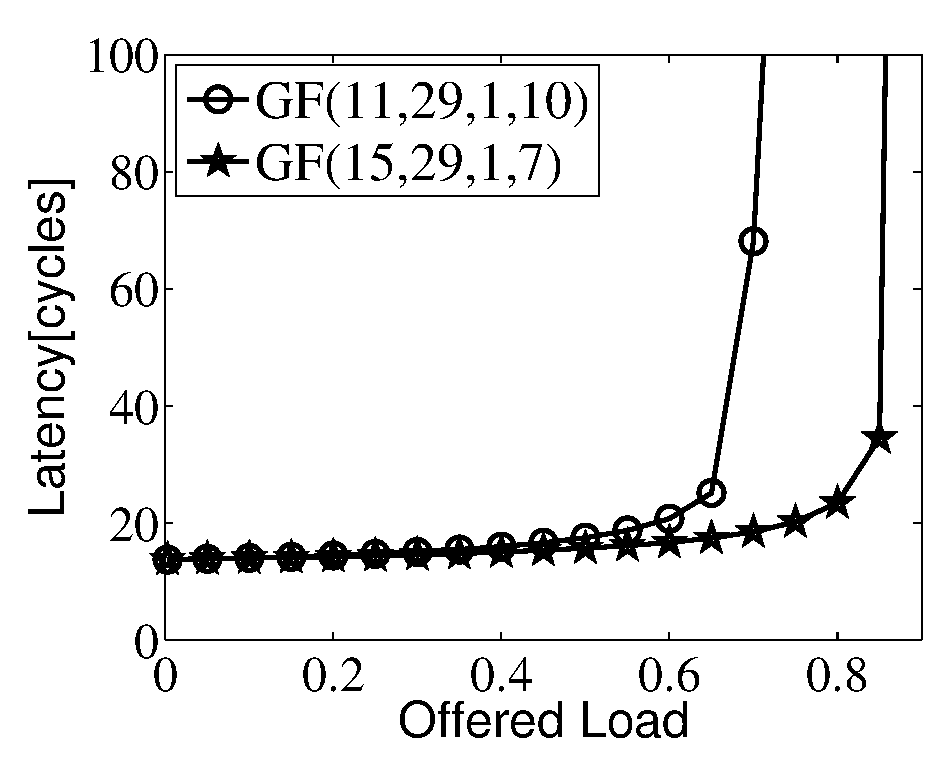
\includegraphics[width=.3\textwidth]{gf_un1.eps}
  \label{gf_un1}
  }
    \subfloat[]{
  \includegraphics[width=.3\textwidth]{gf_un2.eps}
  \label{gf_un2}
  }
    \subfloat[]{
  \includegraphics[width=.31\textwidth]{gf_un3.eps}
  \label{gf_un3}
  }\\
    \subfloat[]{
  \includegraphics[width=.3\textwidth]{gf_un4.eps}
  \label{gf_un4}
  }
    \subfloat[]{
  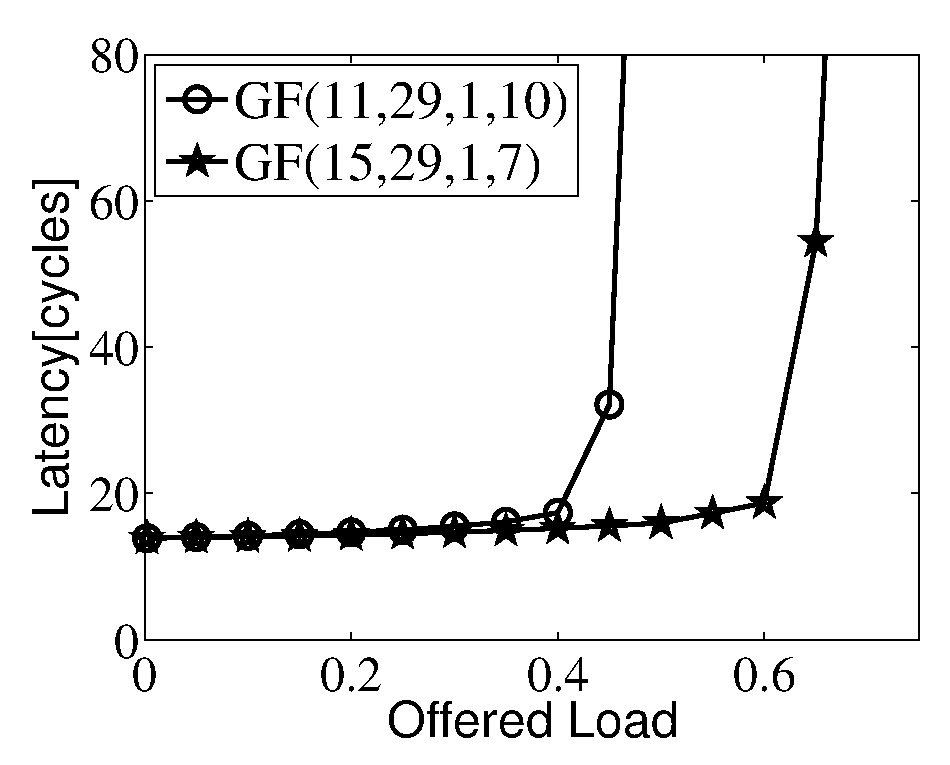
\includegraphics[width=.3\textwidth]{gf_un5.eps}
  \label{gf_un5}
  }
    \subfloat[]{
  \includegraphics[width=.31\textwidth]{gf_un6.eps}
  \label{gf_un6}
  }\\
    \subfloat[]{
  \includegraphics[width=.3\textwidth]{gf_un7.eps}
  \label{gf_un7}
  }
    \subfloat[]{
  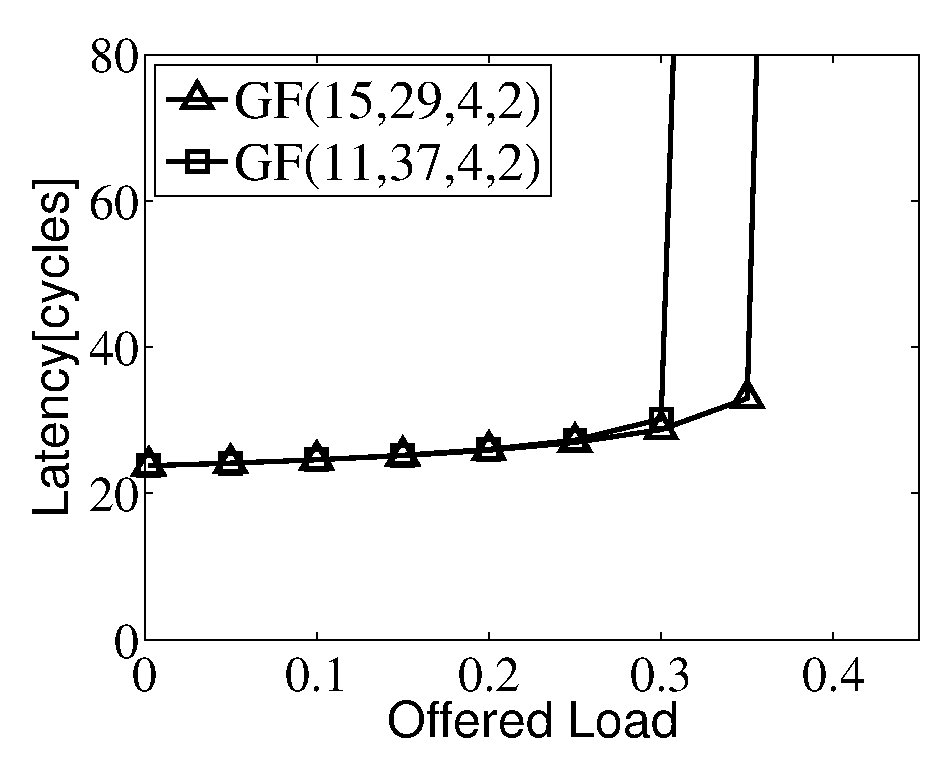
\includegraphics[width=.3\textwidth]{gf_un8.eps}
  \label{gf_un8}
  }
  \caption{不同参数配置的Galaxyfly的性能比较 (a)--(d) 均衡随机通信模式; (e)--(h) 最差情况通信模式。}
  \label{fig:Figure10}
  \end{minipage}
\end{figure*}

\subsubsection{不同的报文长度}

我们分析不同的报文长度如何影响Galaxyfly的网络性能。图\ref{lap3} 和
图\ref{lap4}
展示了不同通信模式下不同报文长度的性能结果。长度越短的报文获得较小的延迟,但是长报文的饱和吞吐率
更高,特别是网络直径较短的Galaxyfly。

\subsubsection{不同的路由算法}

大规模的高性能计算系统,通信模式更加复杂多样。我们引进了一种混合的通信模式去
评测拓扑性能,如图\ref{fig:Figure14}所示。图\ref{lbr2}展示了
GF$(15,29,4,2)$在混合通信模式下四种不同路由算法的性能(其他配置的Galaxyfly也
呈现相似的性能)。NAG算法相比其他路由算法展现了较好的性能。在图\ref{lbr3}
中,不同配置GF的NAG算法获得比MIN算法分别高25\%, 260\%, and 100\%的饱和吞吐率。

\begin{figure}[t]
  \centering
  \begin{minipage}[t]{\textwidth}
   \centering
  \subfloat[]{
  \includegraphics[width=.42\textwidth]{df_un1.eps}
  \label{df_un1}
  }
    \subfloat[]{
  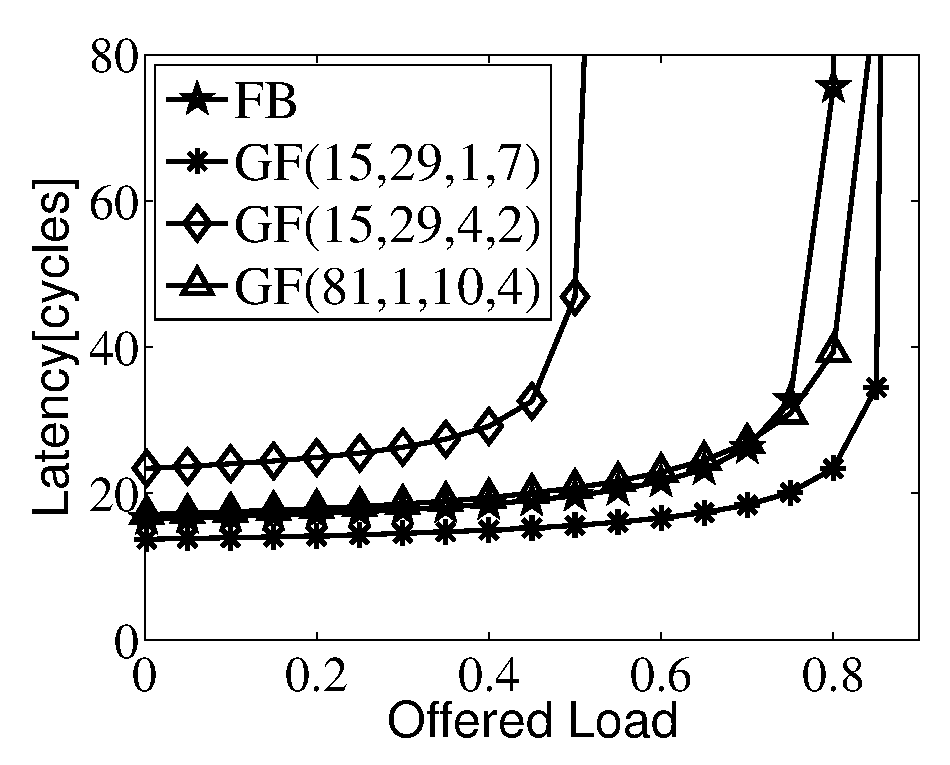
\includegraphics[width=.42\textwidth]{df_un2.eps}
  \label{df_un2}
  }\\
    \subfloat[]{
  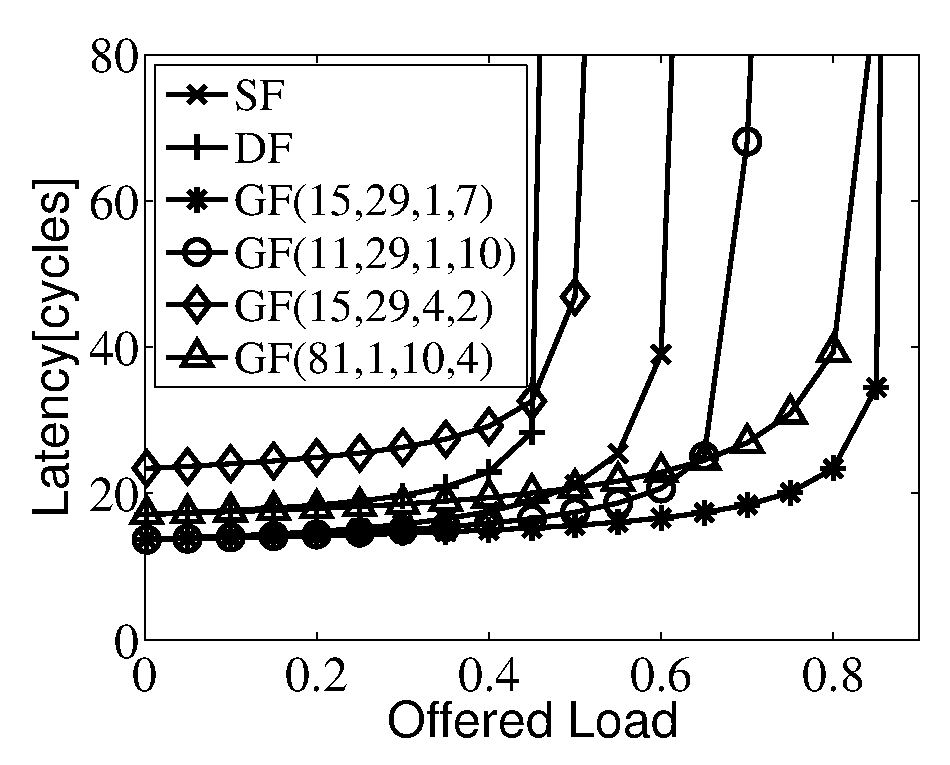
\includegraphics[width=.42\textwidth]{df_un3.eps}
  \label{df_un3}
  }
    \subfloat[]{
  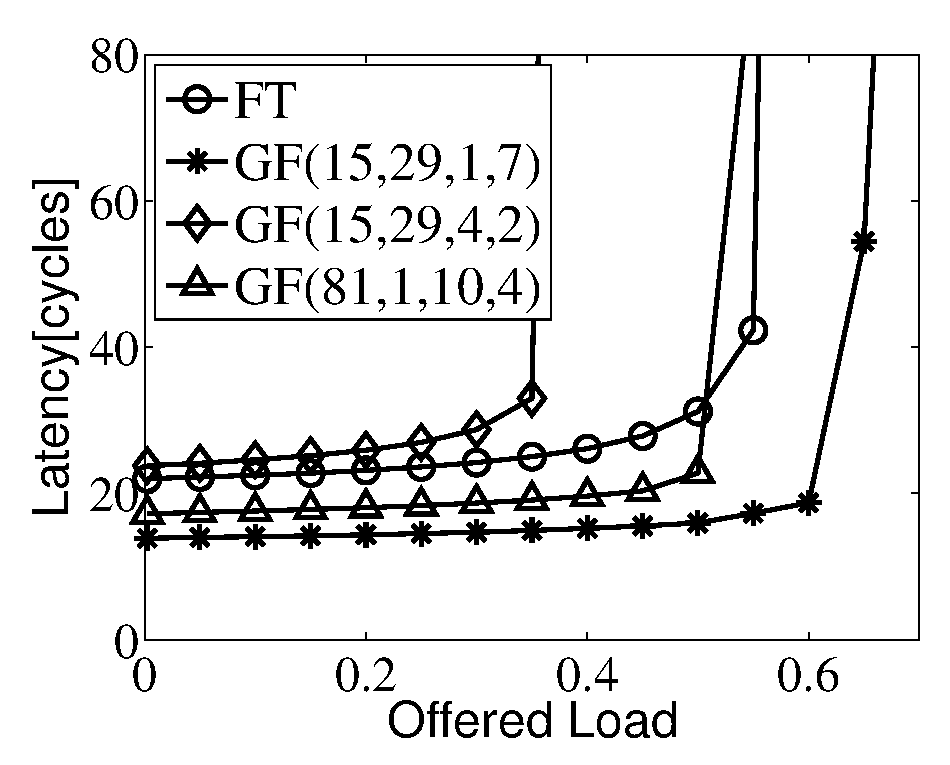
\includegraphics[width=.42\textwidth]{df_un4.eps}
  \label{df_un4}
  }\\
    \subfloat[]{
  \includegraphics[width=.42\textwidth]{df_un5.eps}
  \label{df_un5}
  }
    \subfloat[]{
  \includegraphics[width=.42\textwidth]{df_un6.eps}
  \label{df_un6}
  }
  \caption{不同拓扑结构的性能比较。 (a)--(c) 均衡随机通信模式; (d)--(f) 最差通信模式。}
  \label{fig:Figure11}
  \end{minipage}
\end{figure}

\subsection{不同拓扑结构的比较}

\subsubsection{与Fat tree的比较}
在这一小节中将要详细分析Galaxyfly和Fat tree的性能。
图\ref{df_un1}和图\ref{df_un4}展示了
GF$(15,29,1,7)$的性能比Fat tree的性能更好,但是GF$(15,29,1,7)$
的路由器数量只是Fat tree的64\%。GF$(15,29,1,7)$
的性能优于Fat tree有两个原因,一是因为网络直径更短。
GF$(15,29,1,7)$的网络直径为2而且降低了头阻塞的概率。
Fat tree的长路径路由增加了头阻塞的概率并影响网络的性能。
第二个原因则是较高的全局链路密度。GF$(15,29,1,7)$的
每一个路由器提供80\%的端口给互连同一个集群或者其他集群的
其他路由器。我们也比较了Fat tree和其他拓扑配置。尽管路由器数量
高于Fat tree的路由器数量,但是GF$(81,1,10,4)$的路由器端口数和
GF$(15,29,4,2)$的都要小于Fat tree的路由器端口数。GF$(81,1,10,4)$的路由器端口数
是21,只有Fat tree的70\%。而且,GF$(81,1,10,4)$的网络直径为3,在零负载条件下
也优于Fat tree。GF$(15,29,4,2)$的网络直径为5,在零负载下略高于Fat tree。 但是,
GF$(15,29,4,2)$的路由器端口数只有12,只是Fat tree的40\%。

\subsubsection{与Flattened Butterfly的比较}
我们也比较了Galaxyfly和Flattened Butterfly的性能差别。Flattened Butterfly
是一个高阶的$k-ary$ $n-cube$结构。每一维上是一个全互连的网络。相比Fat tree,
Flattened Butterfly的路由器数量和链路数更少。图\ref{df_un2}和图
\ref{df_un5}
展示了Galaxyfly和3维Flattened Butterfly的性能。
在均衡随机通信负载下,Flattened Butterfly的性能跟GF$(81,1,10,4)$
的相近。两个结构有一样的网络直径。尽管Flattened Butterfly提供了
多于GF$(81,1,10,4)$36\%的全局链路(Flattened Butterfly第一维的结构和
GF$(81,1,10,4)$的超级节点被认为是本地组),Flattened Butterfly的
全局链路分布集中在每一维上,而不是分布在整个全局网络上。另外,
在最差通信模式下,
Flattened Butterfly的饱和吞吐率分别低于GF$(15,29,4,2)$和GF$(81,1,10,4)$
的62.5\%和70\%。


\begin{figure*}[t]
  \centering
    \begin{minipage}[t]{\textwidth}
   \centering
  \subfloat[Uniform random traffic pattern]{
  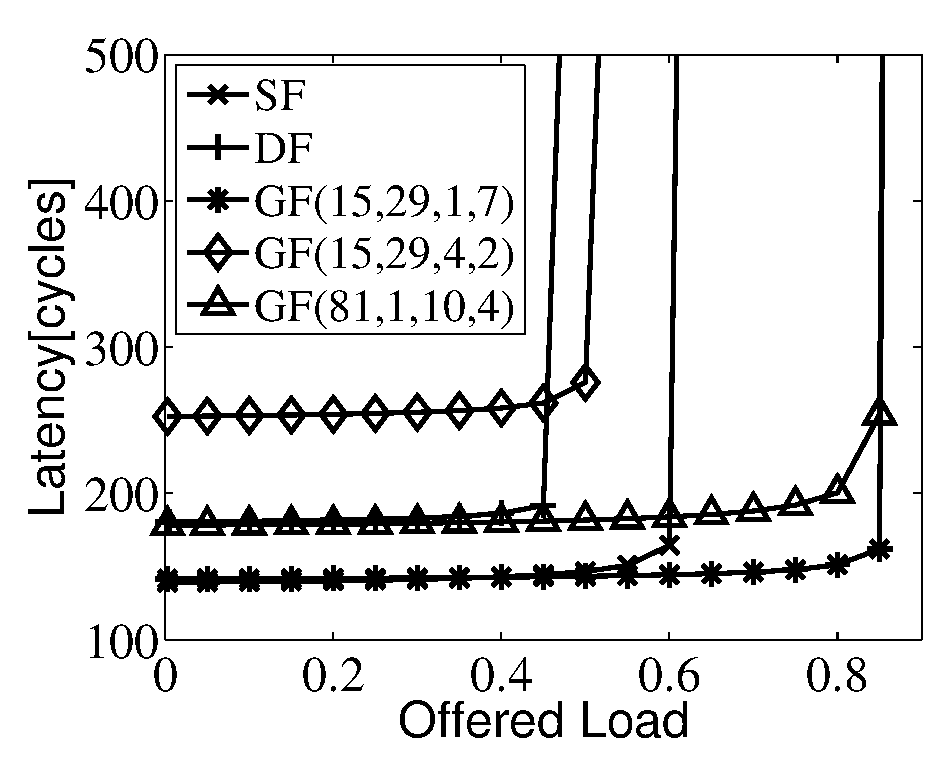
\includegraphics[width=.4\textwidth]{lap1.eps}
  \label{lap1}
  }
    \subfloat[Worst-case traffic pattern]{
  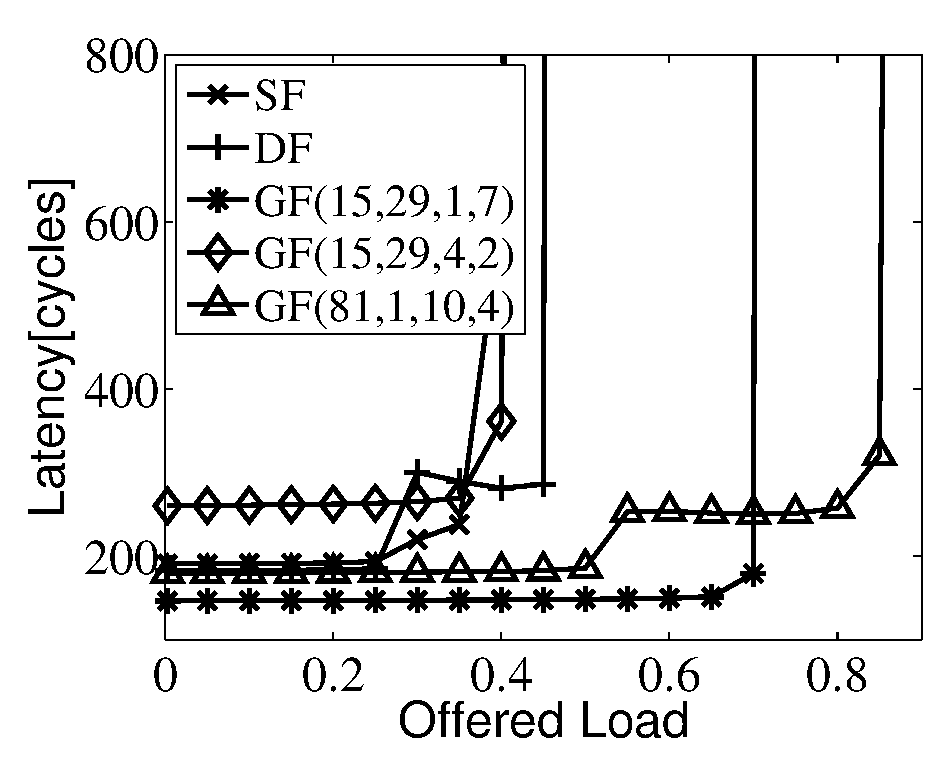
\includegraphics[width=.4\textwidth]{lap2.eps}
  \label{lap2}
  }\\
    \subfloat[Uniform random traffic pattern]{
  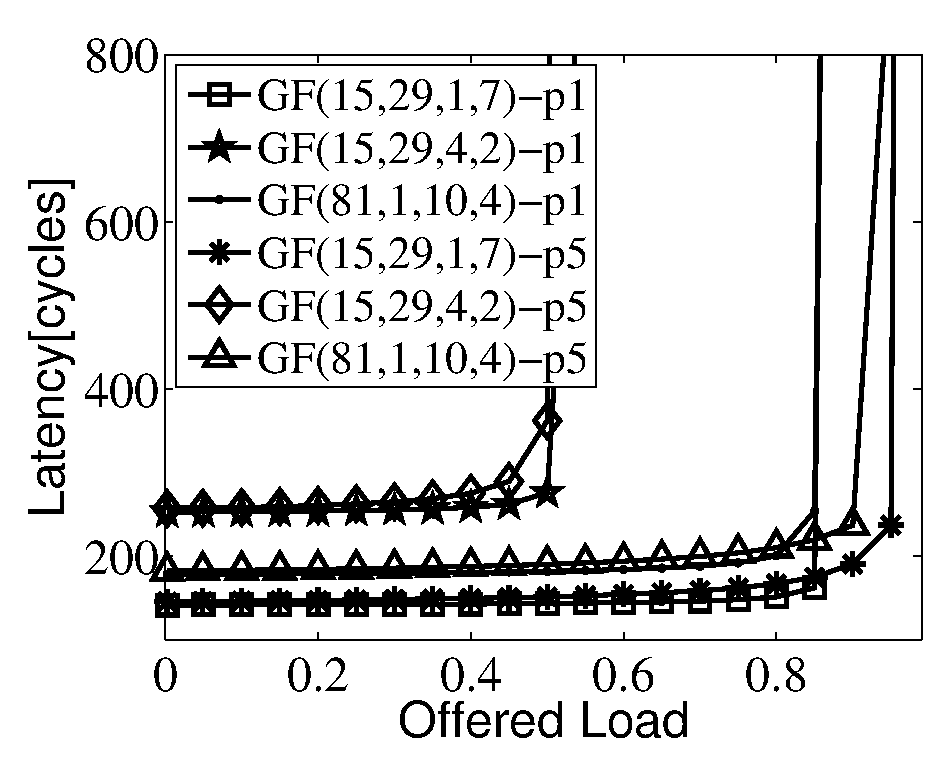
\includegraphics[width=.4\textwidth]{lap3.eps}
  \label{lap3}
  }
    \subfloat[Worst-case traffic pattern]{
  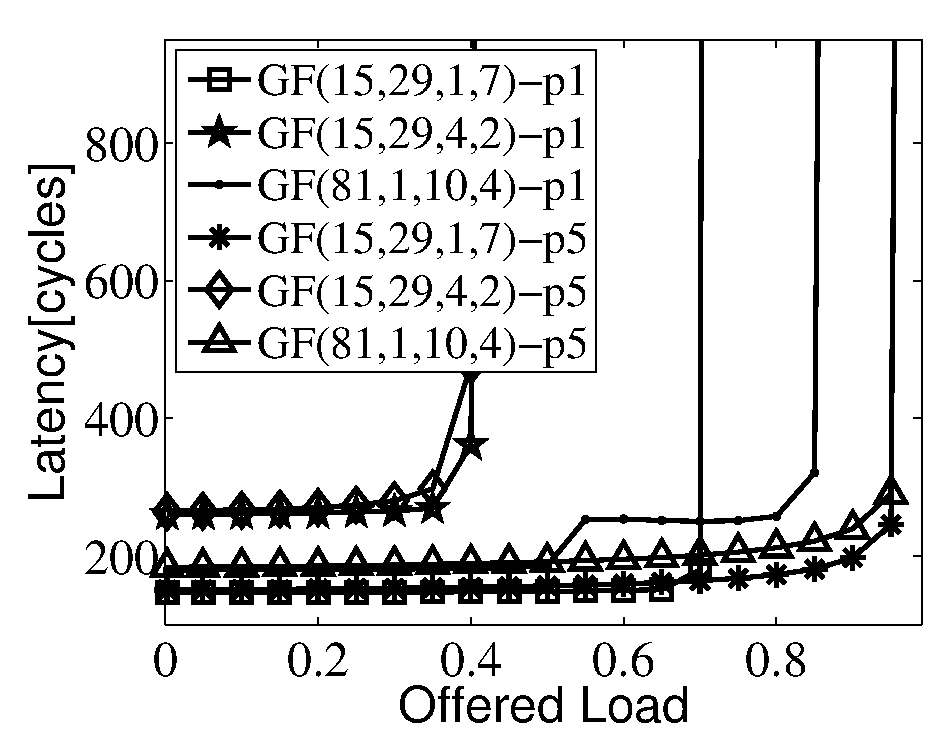
\includegraphics[width=.41\textwidth]{lap4.eps}
  \label{lap4}
  }
  \caption{ 固定物理布局的性能比较(a)--(b). Galaxyfly在不同报文长度下的性能比较(c)--(d)}
  \label{fig:Figure12}
  \end{minipage}
\end{figure*}

\subsubsection{与Slim Fly和Dragonfly的比较}

Slim Fly是最新提出的低直径高性能计算机系统拓扑结构。
Slim Fly跟Galaxyfly一样也利用了代数图论有限域的方法。但是,
Slim Fly的低直径属性是利用了路由器之间相连的端口数$k'$和路由器
规模$N_r$的最优关系,$k'\geq\Omega(\sqrt N_r)$。这个条件严格限制了
Slim Fly的扩展性。相比较,Galayxyfly在使用固定的路由器端口数,
能够构造任意大规模系统。GF(n,q,1,p)也是一个直径为2的拓扑结构。
相比较Slim Fly,在同样网络规模和相近的二分带宽要求下,GF(n,q,1,p)
需要端口数更多的路由器。比如,在表\ref{Table6}中,GF$(11,29,1,10)$
和Slim Fly都是相似的$\beta$,但是GF$(11,29,1,10)$的每一个路由器要求
更多的端口数。GF$(15,29,1,7)$ 是另外一个直径为2的配置,$\beta$值更高以及
路由器端口数更多。因此,在Slim Fly和Galaxyfly的多种配置间中的选择,实际上
是性能和路由器端口数的权衡。图\ref{df_un3}和图\ref{df_un6}
展示了Slim Fly和Galaxyfly不同配置的性能。在均衡随机通信模式和最差通信模式下,
GF$(15,29,1,7)$的性能分别优于Slim Fly的42\%和140\%。GF$(15,29,1,7)$的性能
更优好似因为多于Slim Fly的28\% 路由器和89\%的全局链路。GF$(11,29,1,10)$则
优于Slim Fly的8\%和60\%,也是因为网络中更多的链路。GF$(81,1,10,4)$是直径为3
的结构,零负载延迟略高于Slim Fly。但是,在上述两种通信模式下,
饱和吞吐率则高于Slim Fly将近33\%和100\%。 而且,GF$(81,1,10,4)$的路由器端口数
只是21,约为75\%Slim Fly的。

通常认为,Dragonfly结构是GF$(56,1,11,5)$。Galaxyfly不仅参数配置更加灵活
而且能调整参数获得更好的网络性能。GF$(81,1,10,4)$中每个路由器的端口数
只比Dragonfly结构的路由器多5\% 的端口,但是,性能在任一通信模式下都能优于
Dragonfly的一倍。尽管GF$(15,29,4,2)$的零负载延迟高于Dragonfly,但是
在均衡随机通信模式下,GF$(15,29,4,2)$利用更少得路由器端口获得相似的性能。
而在最差通信模式下,GF$(15,29,4,2)$优于Dragonfly是因为在两个集群之间有
更多的全局链路。

\subsection{物理布局}

我们根据物理布局给布局中的本地链路和全局链路赋
不同的延迟值。

Galaxyfly是一个灵活的层次化结构,由多个集群组成。每一个集群都有同样数目的超级节点
而且集群之间的连线数目相同。Galaxyfly的模块化结构对物理布局有重要意义。
如果超级节点规模过于小,那么可以以一个集群为封装单位即一个集群为一个机柜。机柜
之间有多条链路,可以通过捆绑的方式连接。
否则,就是以一个或多个超级节点封装在一个机柜内使得机柜间有多条链路便于捆绑。
捆绑缆线不仅可以减少缆线成本开销还易于部署\upcite{Jupiter}。


\begin{figure*}[t]
 \begin{minipage}[t]{\textwidth}
   \centering
  \subfloat[GFs、SF和DF的性能比较]{
  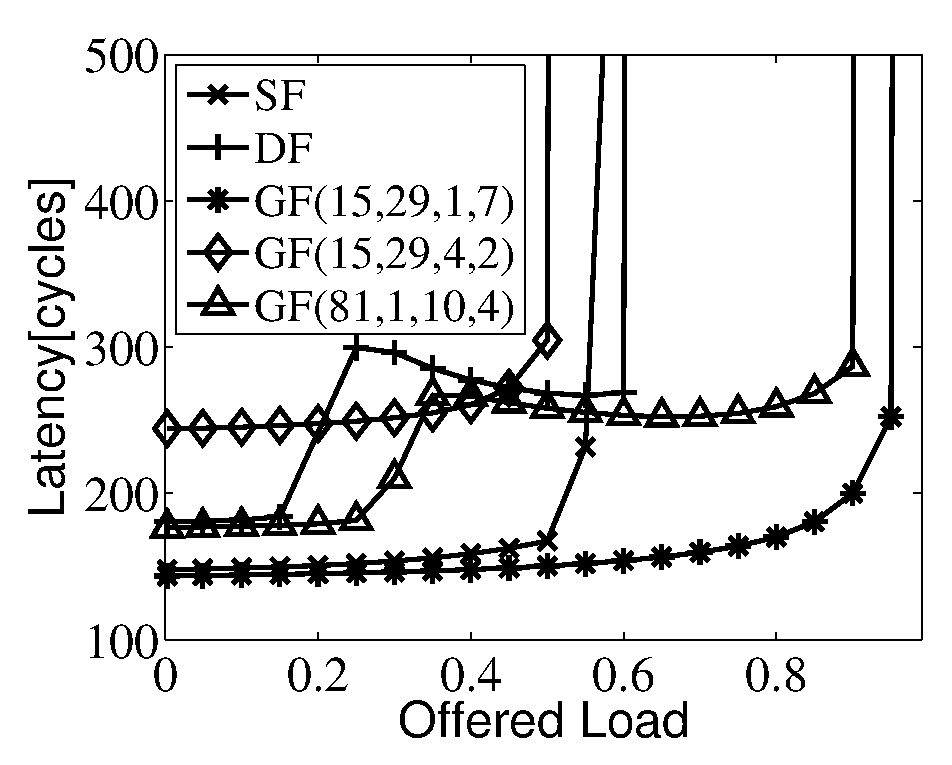
\includegraphics[width=.43\textwidth]{lbr1.eps}
  \label{lbr1}
  }
   \subfloat[不同的路由算法在GF$(15,29,4,2)$的性能]{
  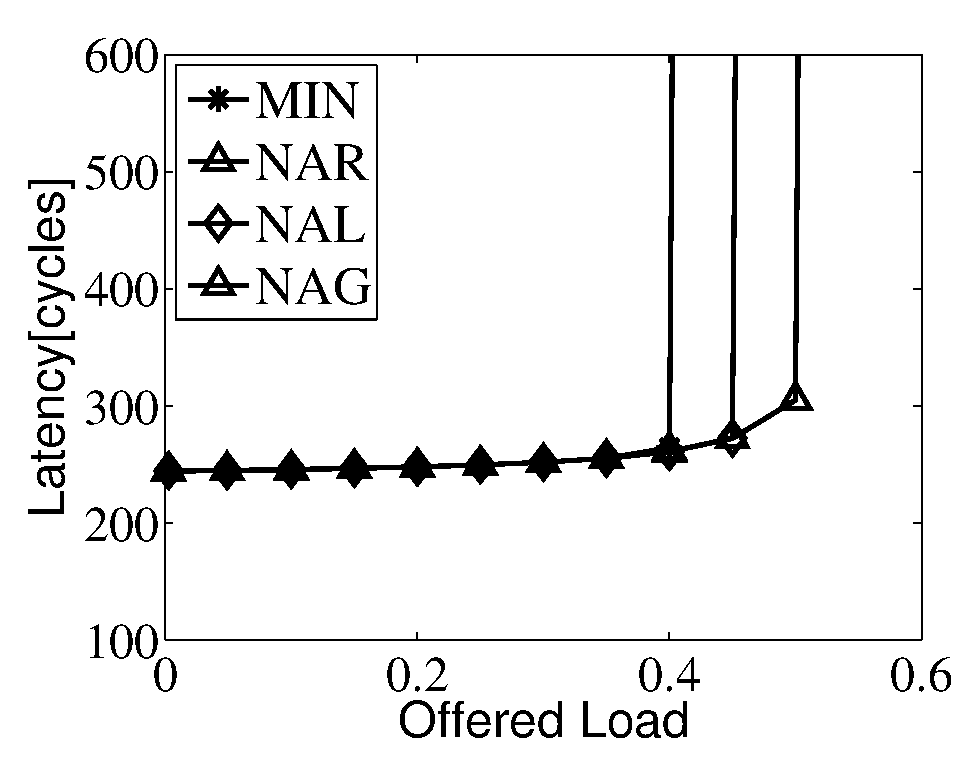
\includegraphics[width=.44\textwidth]{lbr2.eps}
  \label{lbr2}
  }\\
    \subfloat[MIN和NAG的性能比较]{
  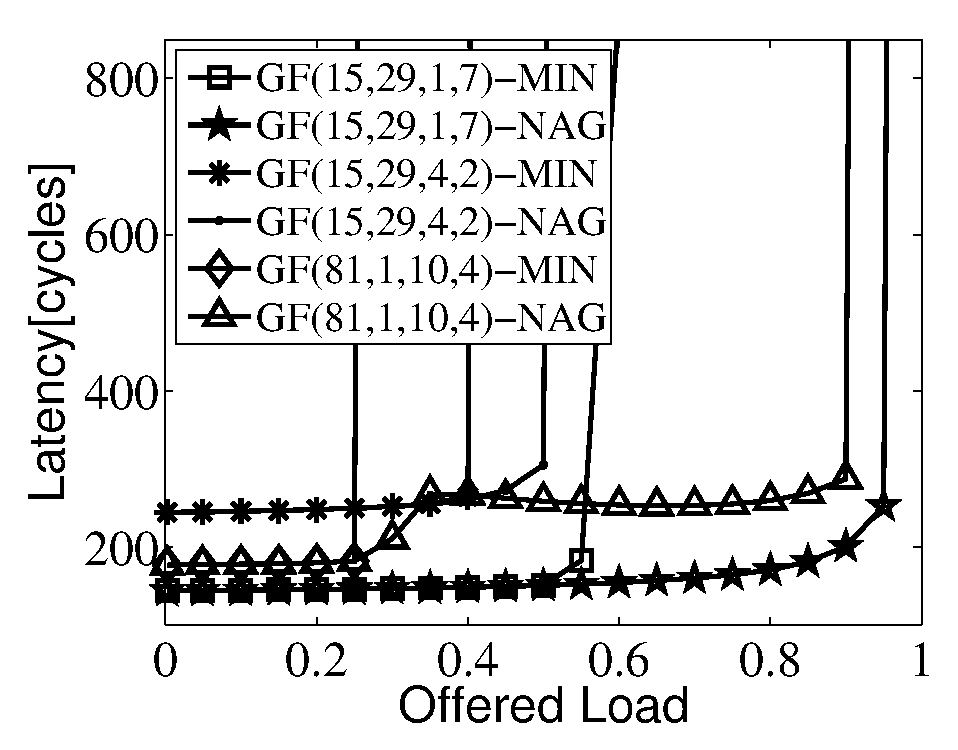
\includegraphics[width=.44\textwidth]{lbr3.eps}
  \label{lbr3}
  }
  \caption{混合通信模式}
  \label{fig:Figure14}
  \end{minipage}
\end{figure*}

Slim Fly和Dragonfly结构都可以看成是层次化结构。他们的布局都类似Galaxyfly。
设置每个机柜都存放200\-360个终端。机柜内的连线使用电信号约50 个时钟周期。
由于光缆的传输速率和频率,机柜之间的全局链路的平均延迟则设为100个时钟
周期。这里提到的延迟都涵盖了报文穿过路由器模块的延迟。

Slim Fly和Dragonfly分别分布在10个和14个机柜内。
GF$(15,29,4,2)$、GF$(15,29,1,7)$ 和GF$(81,1,10,4)$
则分别分布在15、15和9个机柜内。
图\ref{lap1}和图\ref{lap2}展示
了Galaxyfly、Slim Fly和Dragonfly在固定物理布局下的
网络性能。当比较不同的链路延迟和相同的链路延迟的
模拟结果时,网络直径对不同的链路延迟影响效果大。
GF$(15,29,4,2)$因为网络直径最大,其零负载延迟高于其他拓扑结构。
相比GF$(15,29,1,7)$结构,GF$(81,1,10,4)$的饱和
吞吐率与之相近并略好一点,主要是因为GF$(81,1,10,4)$
使用的机柜间链路数量多于GF$(15,29,1,7)$的59.6\%。
GF$(15,29,1,7)$和GF$(81,1,10,4)$的性能都比Slim Fly和Dragonfly
的性能好。我们引进一种混合的通信模式评测Galaxyfly、Slim Fly 和
Dragonfly的性能,如图\ref{fig:Figure14}所示。GF$(15,29,1,7)$
不仅获得最高的饱和吞吐率而且延迟最低,如图\ref{lbr1}所示。
分别在注入率0.25和0.35附近,Dragonfly和GF$(81,1,10,4)$的延迟
突然增加,主要原因是最短路径路由切换到非最短路径路由。


\section{成本和能耗开销}
在本节分析了Galaxyfly和其他拓扑结构在构建网络的两个重要
方面:(1)路由器和缆线的成本开销(2)能耗开销。

拓扑结构的计算节点、路由器以及缆线在实际系统部署时被部署成一个2维的矩形
框架中。在部署过程中一个主要关心的问题是如何使用最少的链路开销部署
低直径网络。一个好的拓扑结构物理部署能大大提升系统的布线效果。

Galaxyfly的结构特性非常适合划分成若干个模块。每一个机柜内都部署
一定的路由器和所连接的终端并使得机柜之间的链路数基本相等。Galaxyfly
可以按集群或者超级节点进行划分。因此,Galaxyfly可以采用合适的参数
$n$、 $q$、 $a$和$p$之间的关系来控制整个系统的成本开销。

\subsection{成本模型}

我们引进一个成本分析模型(类似于\upcite{slimfly}和\upcite{Flattenedbutterfly} 中
使用的模型)来分析整个系统的成本开销,系统的主要开销集中在路由器和互连的缆线上。
假设路由器和终端被封装在一个1 $\times$ 1 $\times$ 2米的机柜中。机柜内的缆线
使用电信号缆线(如背板资源)而机柜间缆线则使用光缆。为了计算缆线的长度,保守
假设机柜内的缆线长度平均约为1\-1.5米长,机柜间的缆线长度则使用3维立方体的
曼哈顿距离估算得到\upcite{slimfly}。在确定机柜数$c$ 的情况下,为了均衡缆线长度,假设机柜
的布局为一个$x\times y+z$的矩形框。每一条机柜间缆线的距离还要额外加上2米的机柜内的开销。

我们比较了Galaxyfly、Dragonfly、Regular Random结构(RR)\upcite{acaserandom}、
Flattened Butterfly(3维)、Fat tree(3层)和Slim Fly的成本开销。为了评估
每个拓扑的成本开销,使用了缆线和路由器的实际价格\upcite{colf}\upcite{mella}来估算。
具体的价格走势如图\ref{crp1}和图\ref{crp2}所示。各个拓扑结构
在规模为$N\approx30K$的负载均衡配置下具体规模不一致但都保证区别在1--3\% 内。

\begin{figure}[t]
  \centering
  \begin{minipage}[t]{\textwidth}
   \centering
  \subfloat[The trend of cable cost]{
  \includegraphics[width=.18\textwidth,height=.32\textwidth]{crp1.eps}
  \label{crp1}
  }
    \subfloat[The trend of router cost model]{
  \includegraphics[width=.18\textwidth,height=.32\textwidth]{crp2.eps}
  \label{crp2}
  }
    \subfloat[ Network cable cost with $N\approx30K$]{
  \includegraphics[width=.52\textwidth,height=.32\textwidth]{crp3.eps}
  \label{crp3}
  }
  \caption{成本开销模型}
  \label{fig:Figure15}
  \end{minipage}
\end{figure}

表\ref{Table7}展示了不同拓扑结构的路由器开销。GF$(25,49,1,24)$的路由器端口数是所有比较
的拓扑结构中最大的。但是,GF$(25,49,1,24)$结构是性价比最高的拓扑结构,而且Dragonfly、
Fat tree、Flattened Butterfly 以及Slim Fly的路由器开销都分别比GF$(25,49,1,24)$
的路由器开销贵36.8\%、68.4\%、27.1\%和 2.2\%。尽管GF$(25,49,8,3)$是性价比最低
的拓扑结构,但是,GF$(25,49,8,3)$的路由器端口数只有Dragonfly的$44\%$,Fat tree
的$25.8\%$,Flattened Butterfly的$32.7\%$和Slim Fly 的$26.2\%$。另外,能够调整Galaxyfly
的参数满足路由器开销和路由器端口数的要求。通过调整超级节点的规模$a$,
GF$(25,49,3,8)$、GF$(25,49,4,6)$ 和GF$(25,49,6,4)$能获得
比GF$(25,49,8,3)$较低的路由器开销而且路由器端口数
也小于其他拓扑结构。


\begin{table}[t]
\caption{Galaxyfly和其他拓扑结构的成本和能耗开销模型}
\centering
\begin{tabular}{c| c| c| c |c| c }\hline
 \centering
  Topology	& Terminals & Routers 	& Radix 	& \tabincell{c}{Routers Cost/\\Terminals(dollars)}	& \tabincell{c}{Power per \\terminal (W)} \\\hline
  DF & 29412 & 3268 & 36 & 1130 & 21 \\\hline
  FT & 29791 & 2883 &62 & 1391 & 24\\\hline
  FB & 28561 & 2197 &49 &1050 &21 \\\hline	
  SF & 29160 &1458 & 61 & 844 & 19\\\hline	
  \tabincell{c}{GF$(25,$\\$49,8,3)$} &29400 &9800 &16 &1602 &25 \\\hline
  \tabincell{c}{GF$(25,$\\$49,3,8)$}	&29400 &3675 &26 &936 &19 \\\hline
  \tabincell{c}{GF$(25,$\\$49,4,6)$} &29400 &4900 &21 &1025 &20 \\\hline
  \tabincell{c}{GF$(25,$\\$49,6,4)$}&29400 &7350 &17 &1269 &22 \\\hline
  \tabincell{c}{GF$(25,$\\$49,1,24)$}&29400 &1225 &72 &826 &18 \\\hline
\end{tabular}
 \label{Table7}
\end{table}
我们分析缆线开销时给不同的拓扑结构提出了各自的划分方式。
每个机柜封装规模相近的终端,如Dragonfly封装一个超级节点。
各个拓扑结构的缆线开销如图\ref{crp3}所示。
Dragonfly、Fat tree、Flattened Butterfly、Slim Fly、Regular Random结构
和5个不同配置的Galaxyfly分别被封装在
$13\times13+3$、 $9\times16+12$、$13\times13$、
$13\times12+6$、$13\times13+3$ 和$13\times13+7$的矩阵排列矩形中。
Fat tree的布局不同于其他拓扑结构,因为其是间接拓扑,所以
叶子路由器和终端被封装在$7\times 16+12$的机柜中和不得不考虑叶子
路由器和终端之间的连接关系。由于层次间的大量连线,
Fat tree的光纤开销是所有拓扑结构最高的。Regular Random结构的
路由器端口数和物理布局都跟Dragonfly的一样。但是大量机柜间的
链路使得Regular Random结构的链路开销高于其他直接拓扑结构。
5个不同配置的Galaxyfly详细参数如表\ref{Table7}所示。这5个
Galaxyfly被封装在同一种布局,所以光纤开销一样。这五个Galaxyfly
缆线开销的区别在于机柜内部的链路开销。GF$(25,49,1,24)$是
性价比最高的结构,他的缆线开销比Slim Fly低5\%。

我们也可以划分结构以Galaxyfly 的集群为单位。在不同的物理布局下,
不同拓扑结构的缆线开销趋势一致。Galaxyfly在合适的配置下可以
构造出性价比高的结构。

\subsection{能耗模型}

网络的能耗开销大概占整个系统开销的50\%\upcite{Energy}。
我们采用能耗模型为一个端口4个SerDes且每个端口的能耗约为
2.8瓦特,以及每个计算节点的网口控制器工作能耗为10瓦特。
表\ref{Table7}展示了Galaxyfly 和其他拓扑结构在能耗模型下
的开销。GF$(25,49,1,24)$是能耗开销最小的结构,主要是因为
较少的路由器数量。

\section{本章小结}

高阶互连网络是当前和未来大规模高性能计算系统的主要拓扑结构。
但是,高阶路由器端口数的增长被当前的SerDes面积、Crossbar仲裁以及能耗
开销等问题制约。本章节基于Galaxy图,我们提出一个新的灵活阶数低直径
拓扑结构,Galaxyfly。他不仅能提升拓扑结构的灵活性还能解决使用较少端口数
的高阶路由器搭建不同规模的网络,从P级系统到E级系统甚至更大规模。而且,
我们构造的Galaxyfly可以较好的权衡网络性能、物理布局复杂度和成本能耗开销
之间的关系。
